\chapter{Der optiboot Bootloader für AVR Mikrocontroller}

\section*{}
Der optiboot Bootloader wurde in der Sprache C von Peter Knight und
Bill Westfield entwickelt. Die Version 6.2 habe ich als Basis
für die hier beschriebene überarbeitete Assembler Version benutzt.
Dabei möchte ich betonen, daß ich den optiboot Bootloader nicht
neu erfunden habe, sondern lediglich weiter optimiert. 
Viele Anpassungen an verschiedene Zielprozessoren und spezielle
Platinenentwürfe waren bereits in der Version 6.2 vorhanden.
Es werden Teile des STK500 Kommunikations-Protokols benutzt,
die in der AVR061~\cite{stk500} von Atmel veröffentlicht wurde.


\section{Änderungen und Weiterentwicklung von Version 6.2}
Im wesentlichen habe ich das komplette Programm in die Assembler-
Sprache umgeschrieben und mit einem bash Shell Script die Erzeugung
der .hex file so umgebaut, daß die Programmlänge
automatisch weiterverarbeitet wird und damit die Startadresse
des Bootloaders sowie die Fuses des ATmega richtig eingestellt werden.
Die eingeschlagene Lösung erzeugt während der Abarbeitung der Einzelschritte
für die Erzeugung des Programmcodes für den Bootloader Variablen,
welche in den nachfolgenden Schritten für die Anpassung
der Start-Adresse und der Fuses erforderlich sind.
Die Startadresse für den jeweiligen Zielprozessor ist abhängig von
der vorhandenen Flash-Speichergröße,
dem Speicherbedarf für den aktuellen Bootloader-Code und
der Kachelgröße, die für Bootloader beim Zielprozessor zur Verfügung steht.
Als Kachelgröße bezeichne ich die kleinste Speichergröße für Bootloader,
die der jeweilige Prozessor zur Verfügung stellen kann.


Bei Prozessoren wie der ATtiny84, die keine Bootloader Startadresse einstellen können,
wird die Seitengröße des Flash-Speichers für die Berechnung benutzt.
Beim ATtiny84 sind das 64 Bytes. Damit liegt die Startadresse des Bootloaders immer
am Anfang einer Flash Speicherseite. 

Bei allen anderen Zielprozessoren kann der Bootloader-Bereich mit den
Fuse-Bits BOOTSZ1 und BOOTSZ0 eingestellt werden (jeweils mit den Werten 0 und 1).
Wenn man die beiden Bits zusammensetzt, ergibt sich daraus die
Bootloader-Größe BOOTSZ mit Werten zwischen 0 und 3.
Dabei bedeutet 3 immer den kleinsten mögliche Bootloader Speicherbereich.
Der Wert 2 gibt den doppelten, der Wert 1 den vierfachen und
der Wert 0 den acht-fachen Speicherbereich vor.
Die Tabelle~\ref{tab:bootsz} auf Seite~\pageref{tab:bootsz} gibt einen
Überblick für verschiedene Zielprozessoren.
Das Bild~\ref{fig:PlatinesAndAVRs} zeigt fast alle Testplatinen und Prozessoren,s
die für die optiboot Tests verwendet wurden. 

\begin{figure}[H]
\centering
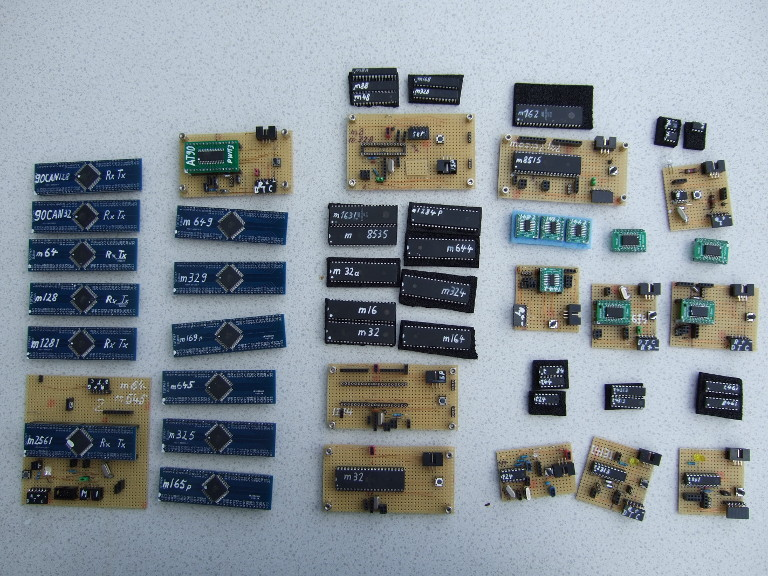
\includegraphics[width=9cm]{../FIG/Samples_AVR_boot.jpg}
\caption{Einige Testplatinen und AVRs für den optiboot Test}
\label{fig:PlatinesAndAVRs}
\end{figure}


\section{Eigenschaften der Assemblerversion von optiboot}

Um viele Fallstricke bei der Erzeugung eines lauffähigen Bootloaders zu umgehen,
wurde die Erzeugung der Bootloader Datei weitgehend automatisiert.
Zusätzlich werden Einstellungen auch geprüft und die Erzeugung mit
einer entsprechenden Fehlermeldung abgebrochen,
wenn beispielweise die gewählte Betriebsfrequenz (AVR\_FREQ) nicht zu der
mit den Fuses (CKSEL,CKDIV8) eingestellten Möglichkeiten für den Takt paßt.
Ein Empfang von Programmdaten für optiboot ist derzeit nur über eine serielle Schnittstelle möglich.\\

Hier sind einige der Fähigkeiten des optiboot Programms aufgelistet:

\begin{itemize}

\item {Unterstützt eine große Zahl von AVRs, wobei fast alle auf Funktion getestet wurden.}

\item {Unterstützt das Laden von Daten in den EEprom Speicher.}

\item {Passt in den meisten Fällen in 512 Byte Flash-Speicher.}

\item {Die Anpassung der Programmgröße und die Änderung der notwendigen Fuses wird automatisch vorgenommen.}

\item {Die von der Programmgröße und dem AVR Modell abhängige Startaddresse wird
	automatisch berechnet und auf dem Bildschirm angezeigt.}

\item {Alle beim jeweiligen AVR-Prozessor vorhandenen seriellen Schnittstellen
	können frei gewählt werden. Als Standard wird immer das erste UART
	benutzt.}

\item {Kann die serielle Schnittstelle über Software emulieren.
	Damit werden auch ATtiny Prozessoren ohne UART unterstützt.
	Außerdem können die TX und RX Pins bei SOFT\_UART völlig frei gewählt werden.}

\item {Bei der SOFT\_UART Lösung kann die serielle Kommunikation auch über nur einen AVR Pin 
	durchgeführt werden. Bei Benutzung des Hardware UARTs ist das nicht sinnvoll, da RXD und TXD Pin
	hier fest vergeben sind.}

\item {Kann eine automatische Baudraten-Anpassung vornehmen.
	Dabei wird die Baudzeit aus dem ersten empfangenen Datenbyte gemessen. 
	Verschiedene Methoden der Baudzeit-Messung können dabei ausgewählt werden.
	Wenn der so konfigurierte optiboot noch in 512 Byte Flash passen soll,
	muß die LED Blink Funktion beim Programmstart abgewählt werden.}

\item {Kann auch für AVRs ohne Bootloader Unterstützung benutzt werden.\\
	Diese VIRTUAL\_BOOT\_PARTITION Fähigkeit kann natürlich auch
	für AVRs benutzt werden, die die Bootloader Unterstützung besitzen.
	Das optiboot Programm wird dabei größer, kann aber dann auf jeder
	Flash-Speicher Seite starten.}

\item {Läßt eine angeschlossene LED standardmäßig drei mal blinken (LED\_START\_FLASHES=3).
	Bei eintreffenden seriellen Daten wird das Blinken aber sofort abgebrochen.}

\item {Anstelle des LED-Blinkens beim Start kann man auch die LED aufleuchten lassen, wenn 
	auf serielle Daten gewartet wird (LED\_DATA\_FLASH=1).
       Auch ein Dauerleuchten der LED kann mit LED\_DATA\_FLASH=4 gewählt werden.
       Dabei geht die LED erst durch den Watchdog-Reset wieder aus.}

\item {Die Länge des erzeugten Programms ist nur abhängig vom gewählten AVR-Prozessor
	und den ausgesuchten Optionen.
	Die Version des avr-gcc Kompilers spielt keine Rolle wenn die Assembler Quellen benutzt werden.
	Dies macht eine nachträgliche Kontrolle (Verify) des installierten Bootloaders
	einfacher, selbst mit einem anderen PC.}

\item {Unterstützt die Anpassung der Oszillator-Frequenz für den AVR internen RC-Oszillator.
 	Dadurch ist auch in Problemfällen die Benutzung eines Bootloaders mit fester Baudrate möglich.}

\item {Das Laden des optiboot Programms in den jeweiligen AVR Prozessor kann automatisch mit dem
	Programm avrdude und einem angeschlossenem ISP-Programmer erfolgen.
	Dazu ist nur die zusätzliche Eingabe von ISP=1 beim make Aufruf erforderlich.
	Die zusätzliche Eingabe ISP=2 würde eine Verifikation mit avrdude bewirken.
	Mit ISP=3 wird der gesamte Programmspeicher (Flash) des angeschlossenen AVR ausgelesen.
	Mit ISP=4 wird der gesamte EEprom-Speicher des angeschlossenen AVR ausgelesen.}

\end{itemize}

Die nachfolgenden Fähigkeiten beziehen sich nur auf den Herstellungsprozess des Bootloaders:

\begin{itemize}

\item {Für die Erzeugung des optiboot Bootloaders können wahlweise auch angepaßte C-Quellen
	benutzt werden. Die meisten Funktionen sind auch hier möglich.
	Natürlich wird das erzeugte optiboot Programm größer!}

\item {Der Umfang der Bildschirmausgabe bei der Erzeugung von optiboot kann mit der Systemvariablen
	VerboseLev verändert werden. Der Wert kann zwischen 1 und 4 liegen, wobei 2 der Standardwert ist.}

\item {Die Bildschirmausgabe kann mit der Systemvariablen WITH\_COLORS=1 bunter gestaltet werden.
	Mit WITH\_COLORS=2 wird reiner Text ausgegeben}

\item {Die Erzeugung des optiboot Programms wird in einer Bash Script Datei gesteuert, wobei die
	Text-Datei avr\_params.def die notwendigen Daten für alle unterstützten AVR-Prozessoren liefert.
	In dieser avr\_params.def Datei sind auch für jeden unterstützten Prozessor Standard-Werte
	für die Fuses, Arbeitsfrequenz und Baudrate festgelegt.}

\item {Die für die jeweiligen Prozessoren verfügbaren Pinbelegungen findet die Script Datei 
	in dem avr\_pins Verzeichnis in einer passenden Datei. Hier werden bei Bedarf auch
	Standardwerte für die von SOFT\_UART benutzten Pins und für die LED gefunden.}

\item {Die Erzeugung des optiboot Programms läuft unter Linux mit installierten avr Paketen.
	Eine Erzeugung unter Windows10 ist möglich,
	wenn zusätzlich zum Arduino Paket Programmpakete installiert sind,
	die die bei der Erzeugung erforderlichen Programme wie bash, bc, echo und andere zur Verfügung stellt.
	Geprüft habe ich das Cygwin64 Paket auf einen Windows10 Laptop mit vorher installierten Arduino Paket.}

\item {Die bei der Programmerzeugung gewählten Parameter werden sowohl am Ende einer .lst Datei
	als auch in einer .log Datei festgehalten.}

\end{itemize}

\section{Automatische Größenanpassung in der optiboot Makefile}

Die Bootloader Startadresse und die benötigte Bootloadergröße wird
automatisch in dem von der Makefile aufgerufenem bash script build\_hex.sh angepasst.
Für die Berechnungen werden einige Variable erzeugt, was nur zusammen
mit den folgenden Linux Werkzeugen funktioniert:

\begin{description}
\item [bash] ein leistungsfähiger Kommandoprozessor für die Abarbeitung des Scripts. 
\item [bc] ein einfacher Rechner, der die Eingabe- und Ausgabe-Werte
sowohl dezimal als auch sedezimal (hex) verarbeiten kann.
\item [cat] gibt den Inhalt von Dateien auf der Standard-Ausgabe aus.
\item [cut] kann Teile von Zeilen einer Textdatei ausschneiden.
\item [echo] gibt den angegebenen Text auf der Standard-Ausgabe aus.
\item [grep] gibt nur Zeilen einer Textdatei mit dem angegebenen Suchtext aus.
\item [tr] kann Text-Zeichen ersetzen oder löschen.
\end{description}

Bisher ist die Funktion des bash Scipts nur mit einem Linux-System und
unter Windows10 mit installiertem Cygwin Paket zusammen mit den Arduino Paket getestet.

Hier sind die Namen und die Bedeutung der Script Dateien aufgeführt.
\begin{description}

\item [build\_hex.sh] erhält die Variablen von der Makefile, mit der dann ein passender
optiboot Hex-Datei in Intel Format erzeugt wird.
Der build\_hex.sh Script ruft die weitere Shell Scripte  get\_avr\_params.sh,
avr\_family.sh, show\_led\_pin.sh, show\_rx\_pin.sh und show\_tx\_pin.sh auf.
Wenn die Variable ISP gesetzt ist, wird auch der Script program\_target.sh
aufgerufen.

\item [program\_target.sh] wird von build\_hex.sh aufgerufen, um die hfuse und efuse Einstellung
zu überprüfen und zu korrigieren. Bei geänderter Anzahl der benutzten Bootpages
müssen die BOOTSZ Bits des ATmega angepaßt werden. Die Bits liegen je nach AVR-Modell
in dem hfuse oder efuse Byte, was die Korrektur nicht einfacher macht.
Nach erfolgten Korrekturen wird das Programm avrdude mit dem Script only\_avrdude.sh aufgerufen,
um den AVR mit dem optiboot Bootloader zu beschreiben und alle Fuses zu setzen.

\item [only\_avrdude.sh] enthält nur einen avrdude Aufruf mit der in der Variablen
DUDE\_PARAMS Parameterliste. Zur Kontrolle wird der Aufruf auf dem Terminal protokolliert.
Wenn avrdude bei der Rückkehr einen Fehler meldet, gibt der Script allgemeine Hinweise
zur Fehlersuche aus. Bei einem Linux System wird auch nach eventuell passenden 
seriellen Schnittstellen gesucht.

\item [find\_serials.sh] Sucht in einem Linux System nach möglichen Namen für USB-Seriell
Wandlern. Für diese Aufgabe gibt es passende Chips, die auf Linux Systemen meist mit dems
Namen /dev/ttyUSB beginnen.
Es gibt auch Software-Emulationen auf Mikrokontrollern, die eine USB-Schnittstelle
integriert haben. Diese sind meist über einen Namen zugreifbar, der mit /dev/ttyACM beginnt.
Es wird auch für jede gefundene Schnittstelle überprüft, ob ein Zugriff möglich ist.
Dazu muß man als Benutzer in der Gruppe Mitglied sein, der diesen Gerät den Zugriff
erlaubt (meist dialout).
Dieser Script wird von only\_avrdude bei Fehler Rückkehr aufgerufen, man kann den
Script auch mit bash ./find\_serials.sh aufrufen.
Wenn man mit einer bash arbeitet, kann man sie ausführbar machen und direkt aufrufen
mit ./find\_serials.sh.
Bei Windows ist dieser Script nutzlos. Bein Windows muß man den Geräte Manager benutzen.

\item [get\_avr\_params.sh] findet für den mit MCU\_TARGET spezifizierten AVR Prozessor
alle benötigten Parameter wie Flashgröße, die Größe der Flash-Seiten und die Größe einer
Bootloader Seite. Zusätzlich werden auch einige Parameter wie Betriebsfrequenz,
Baudrate und die Belegung der Fuses besetzt, wenn nicht anders vom Nutzer gewünscht.
Die Quelle für diese Vorbesetzungen ist die Datei avr\_params.def .

\item [avr\_family.sh] buildet einen Gruppennamen für AVR-Prozessoren mit gleicher
Pinbelegung. Normalerweise ist der Gruppenname identisch mit dem AVR Prozessorname
mit dem größten Speicher (atmega328 für atmega168 oder atmega88).

\item [show\_led\_pin.sh] findet den Pin für die LED, der für diesen Prozessor
oder die Gruppe als Standard vorgegeben ist und protokolliert diese Wahl
auf dem Terminal. Wenn der Bediener einen anderen Pin gewählt hat, wird dieser
Pin protokolliert.
Ohne die Benutzerwahl wird der Pin aus einer avr\_pins/<group>.pins Datei entnommen.

\item [show\_rx\_pin.sh] protokolliert den gewählten  RX Pin für die eingehenden seriellen Daten.
Ohne eine spezielle Benutzerwahl bei SOFT\_UART wird der Pin aus einer avr\_pins/<group>.pins Datei entnommen.

\item [show\_tx\_pin.sh] protokolliert den gewählten TX Pin für die Ausgabe der seriellen Daten.
Ohne eine spezielle Benutzerwahl bei SOFT\_UART wird der Pin aus einer avr\_pins/<group>.pins Datei entnommen.

\item [baudcheck.tmp.sh] wird während der Abarbeitung von build\_hex.sh durch einen
C-Preprozessor Aufruf aus der Datei baudcheck.S erzeugt und ausgeführt, um Informationen
über die gewählte Baudraten Einstellung zu geben.

\end{description}

\section{Zielvorgaben für optiboot Makefile}

Es können verschiedene Konfigurationen auch für einen Prozessortyp
festgelegt wnd In der Tabelle~\ref{tab:processors} sind die einige der derzeit vordefinierten
Konfigurationen für AVR Prozessoren angegeben. 
Die einstellbaren Parameter sind aber auch in der Aufrufzeile des
make Programms als Parameter oder auch als Umgebungsvariable der Shell
einstellbar und haben Vorrang zu den Grundeinstellungen.
Es gibt zwei Haupt Variabalennamen, die dem bash Script build\_hex.sh übergeben
werden, TARGET und MCU\_TARGET . Die Variable MCU\_TARGET muß dabei
einen legalen AVR Prozessor Name enthalten. Die Variable TARGET kann mit einem frei wählbaren
Namen belegt werden, ist aber üblicherweise identisch dem MCU\_TARGET Namen oder
ist der Name einer Platine mit diesem Prozessor.

\begin{table}[H]
  \begin{center}
    \begin{tabular}{| c | c | c | c | c | c | c | c | c |}
    \hline
             Name  & MCU & AVR\_ & total & Flash & BP\_ & LFUSE & HFUSE & EFUSE  \\
                   &     & FREQ  & Flash & page  & LEN  &       &       &        \\
                   &     &       &  size & size  &      &       &       &        \\
    \hline
    \hline
         attiny84 & t84   & 16M? &  8K   &  64   & (64) &  62   &  DF   & FE \\
    \hline
         atmega8  & m8    & 16M  &  8K   &  64   & 256  &  BF   &  CC   &  - \\
    \hline
         atmega88 & m88   & 16M  &  8K   &  64   & 256  &  FF   &  DD   &  04 \\
    \hline
       atmega16   & m16   & 16M  &  16K  & 128   & 256  &  FF   &  9C   &  - \\
    \hline
       atmega168  &  m168  & 16M  &  16K & 128   & 256  &  FC   &  DD   &  04 \\
       atmega168p &  m168p & 16M  &  16K & 128   & 256  &  FC   &  DD   &  04 \\
    \hline
       atmega32   &  m32   & 16M  &  16K & 128   & 256  &  BF   &  CE   &  - \\
    \hline
       atmega328  &  m328  & 16M  &  32K & 128   & 512  &  FF   &  DE   &  05 \\
       atmega328p & m328p & 16M  &  32K  & 128   & 512  &  FF   &  DE   &  05 \\
    \hline
       atmega644p & m644p & 16M  &  64K  & 256   & 512  &  F7   &  DE   &  05 \\
    \hline
     atmega1284p & m1284p & 16M  & 128K  & 256   & 512  &  F7   &  DE   &  05 \\
    \hline
     atmega1280  & m1280  & 16M  &  128K & 256   & 1K   &  FF   &  DE   &  05 \\
    \hline
    \end{tabular}
  \end{center}
  \caption{einige Prozessor targets für optiboot Makefile}
  \label{tab:processors}
\end{table}

Alle Angaben für Größen sind in Bytes angegeben, die Werte für die Fuses sind die sedezimalen
Werte (hex). Die Frequenz-werte werden in Hz angegeben, 16M entspricht also 16000000 Hz.
Die Standard Baud-Rate für die serielle Schnittstelle beträgt bei \(16 MHz\) Betrieb meistens 115200.

Neben den universellen Konfigurationen gibt es auch Konfigurationen für bestimmte
Platinen oder Arbeitsumgebungen.
Die Tabelle~\ref{tab:boards} zeigt die unterschiedlichen Einstellungen.

\begin{table}[H]
  \begin{center}
    \begin{tabular}{| c | c | c | c | c | c | c | c | c | c | }
    \hline
             Name  & MCU & AVR\_ & BP\_ & L     & H     & E     & BAUD\_ & LED & SOFT\_ \\
                   &     & FREQ  & LEN  &  FUSE & FUSE  &  FUSE & RATE &     & UART \\
    \hline
    \hline
       luminet     & t84 &  1M   & 64v &  F7   &  DD   &  04   & 9600 & 0x  &  -   \\

    \hline
         virboot8  & m8    & 16M & 64v &       &       &       &      &     &      \\
    \hline
       diecimila  &  m168 & (16M) &     &  F7   &  DD   &  04   &      & 3x  &  -   \\
       lilypad    &  m168  & 8M  &      &  E2   &  DD   &  04   &  -   & 3x  &  -   \\
       pro8       &  m168  & 16M &      &  F7   &  C6   &  04   &  -   & 3x  &  -   \\
       pro16      &  m168  & 16M &      &  F7   &  DD   &  04   &  -   & 3x  &  -   \\
       pro20      &  m168  & 16M &      &  F7   &  DC   &  04   &  -   & 3x  &  -   \\
    atmega168p\_lp&  m168  & 16M &      &  FF   &  DD   &  04   &  -   &     &  -   \\
   xplained168pb  &  m168  &(16M)&      &       &       &      & 57600 &     &      \\
    \hline
       virboot328  & m328p & 16M & 128v &       &       &       &      &     &  -   \\
    atmega328\_pro8& m328p & 8M  &      &  FF   &  DE   &  05   &  -   & 3x  &  -   \\
   xplained328pb  &  m168  &(16M)&      &       &       &      & 57600 &     &      \\
   xplained328p   &  m168  &(16M)&      &       &       &      & 57600 &     &      \\
    \hline
        wildfire  & m1284p & 16M &      &       &       &      &   -   & 3xB5 &      \\
    \hline
       mega1280    & m1280 & 16M &      &  FF   &  DE   &  05   &  -   &     &  -   \\
    \hline
    \end{tabular}
  \end{center}
  \caption{vorkonfigurierte targets für optiboot Makefile}
  \label{tab:boards}
\end{table}

\section{Die Optionen für die optiboot Makefile}

Mit den Optionen wird die Eigenschaft des optiboot Bootloaders eingestellt.
Beispielsweise kann mit der Option SOFT\_UART veranlasst werden, daß ein
Softwareprogramm für die serielle Kommunikation verwendet werden soll.
Sonst wird, wenn vorhanden, die auf dem Chip integrierte  serielle Schnittstelle
mit den Pins TX (Transmit = senden) und RX (Receive = empfangen) benutzt.
Bei mehreren integrierten seriellen Schnittstellen wird normalerweise die erste
Schnittstelle mit den Nummer 0 verwendet. Es kann aber auch jede andere vorhandene
Schnittstelle mit der Option UART vorgegeben werden (UART=1 für die zweite Schnittstelle).
Bei der Hardware UART Schnittstelle sind die Pins für Empfangen (RX) und Senden (TX)
fest verknüpft. Bei der Software-Lösung für die serielle Schnittstelle sind alle Pins
des AVR Prozessors frei für die serielle Kommunikation wählbar. Die einzige Bedingung
ist, daß die Pins für digitale Eingabe (RX) beziehungsweise Ausgabe (TX) geeignet sind.
Näheres zu den möglichen Optionen findet man in der Übersicht~\ref{tab:options1}, \ref{tab:options2}
und \ref{tab:options3}

\begin{table}[H]
  \begin{center}
    \begin{tabular}{| c | c | l |}
    \hline
   Name der        & Beispiel       & Funktion                                            \\
    Option         &                &                                                     \\
    \hline
    \hline
    F\_CPU         & F\_CPU=8000000 & Teilt dem Programm die Taktrate des Prozessors mit. \\
                   &                & Die Angabe erfolgt in Hz (Schwingungen pro Sekunde. \\
                   &                & Das Beispiel gibt eine Frequenz von 8 MHz an. \\
    \hline
    BAUD\_RATE     & BAUD\_         & Gibt die Baud-Rate für die serielle Kommunikation an. \\
                   &  RATE=9600     & Es werden immer 8 Datenbits ohne Parity verwendet. \\
                   &                & Werte \textless~100 aktivieren eine Messung and Anpassung \\
                   &                & der Baudrate mit verschiedenen Verfahren.  \\
		   &                & Der Vorteil besteht darin, daß man problemlos auf eine \\
		   &                & niedrigere Baudrate ausweichen kann, wenn Probleme \\
		   &                & mit einer hohen Baudrate auftauchen. \\
    \hline
    SOFT\_UART     & SOFT\_UART=1   & Wählt Software-Lösung für die serielle Kommunikation. \\
    \hline
    UART\_RX        & UART\_RX=D0   & Gibt den Port und die Bitnummer für die seriellen  \\
                   &                & Empfangsdaten an. Das Beispiel nimmt               \\
                   &                & Bit 0 des D Ports für den seriellen Eingang.\\
    \hline
    UART\_TX        & UART\_TX=D1   & Gibt den Port und die Bitnummer für die seriellen  \\
                   &                & Sendedaten an.  Das Beispiel nimmt Bit 1 des D Ports \\
                   &                & für den seriellen Ausgang.\\
    \hline
    UART           & UART=1         & Wählt für die  serielle Schnittstelle des Chips. \\
                   &                & Eine Auswahl setzt das Vorhandensein mehrerer \\
                   &                & Schnittstellen voraus, funktioniert dann aber auch \\
		   &                & mit SOFT\_UART. \\
    \hline
    INVERSE\_UART  & INVERSE\_UART=1 & Invertiert die Pegel von RX und TX Signalen. Die \\
	           &                & Option kann nur bei Software UART benutzt werden.\\
    \hline
 LED\_START\_      & LED\_START\_   & Wählt für die Anzahl der Blink-Zyklen \\
   FLASHES         &   FLASHES=3    & für die Kontroll-LED. Bei 1 oder -1 wird nur einmal \\
                   &                & geblinkt ohne Wiederholung. Negative Vorgaben \\
                   &                & bedeuten, daß in der Programmschleife das RX Bit der \\
                   &                & seriellen Schnittstelle nicht überwacht wird. Bei \\ 
                   &                & positiven Werten wird die Binkschleife sofort \\
		   &                & abgebrochen, sobald eingehende RX-Daten festgestellt \\
                   &                & werden. Bitte beachten Sie,daß das Blinken den Start \\
                   &                & des Anwenderprogramms verzögert. \\
    \hline
 LED               & LED=B3         & Wählt das Port-Bit für die  Kontroll-LED. \\
                   &                & Beim Beispiel würde eine an das Bit 3 des Port B \\ 
                   &                & angeschlossene LED blinken. Bei der \\
                   &                & LED\_START\_FLASHES  Option  blinkt die LED die\\
                   &                & angegebene Anzahl vor dem Kommunikations-Start. \\
    \hline
 LED\_DATA\_       & LED\_DATA\_    & Die Kontroll-LED leuchtet während des Wartens auf \\
      FLASH        &    FLASH=1     & Empfangsdaten der seriellen Kommunikation.\\
	           &                & Ein Wert von 4 bewirkt, daß die LED nur beim Start \\
		   &                & einmalig eingeschaltet wird. Hiermit kann man auch \\
		   &                & erkennen, daß der Bootloader gestartet wurde und \\
		   &                & es wird viel weniger Platz im Programmspeicher \\
		   &                & gebraucht. \\
    \hline
    \end{tabular}
  \end{center}
  \caption{Wichtige Optionen für die optiboot Makefile}
  \label{tab:options1}
\end{table}

Bei Betrieb mit internem RC-Generator ist es durchaus möglich, daß ein serieller Datentransfer
nicht auf Anhieb gelingt. Das ist prinzipiell auch unabhängig davon, ob die Hardware UART
Schnittstelle oder eine Softwarelösung (SOFT\_UART) benutzt wird. Ohne zusätzliche Messungen
ist man dann auf Probieren mit der OSCCAL\_CORR angewiesen. Einen Hinweis kann
das Datenblatt des Prozessors liefern. Hier ist beschrieben, bei welcher Betriebsspannung
und bei welcher Temperatur der RC-Oszillator kalibriert wurde. Außerdem ist der
prinzipielle Verlauf der Frequenzänderung mit der Betriebsspannung, mit der Temperatur und
mit OSCCAL-Änderung beschrieben. 


Weitere Optionen sind in den Tabellen~\ref{tab:options2} und~\ref{tab:options3} aufgezählt. 
Diese Optionen sind meist nur für Software-Untersuchungen, die Frequenzkalibration des RC-Generators
 und für Prozessoren ohne Bootloader-Bereich interessant.

\begin{table}[H]
  \begin{center}
    \begin{tabular}{| c | c | l |}
    \hline
   Name der        & Beispiel       & Funktion                                            \\
    Option         &                &                                                     \\
    \hline
    \hline
 TIMEOUT\_MS       & TIMEOUT\_      & Diese Option gibt eine Zeitschranke in Millisekunden \\
                   &  MS=2000       & vor für den Empfang von Boot-Daten. Nach dieser Zeit\\
                   &                & wird der Bootvorgang abgebrochen und versucht, das \\
                   &                & Anwenderprogramm zu starten. Mögliche Werte für \\
                   &                & TIMEOUT\_MS sind 500, 1000, 2000, 4000 und 8000. \\
                   &                & Der tatsächlich mögliche Wert kann abhängig vom \\
                   &                & Prozessor auf 2 Sekunden begrenzt sein. \\
                   &                & Wenn kein TIMEOUT\_MS angegeben wird, wird die \\
                   &                & Zeitschranke auf 1 Sekunde gesetzt. \\
    \hline
    SUPPORT\_      & SUPPORT\_      & Wählt für das Bootloader-Programm die Lese- und Schreib- \\
    EEPROM         &  EEPROM=1      & Funktion für EEproms. Wenn als Quelle das Assembler- \\
                   &                & Programm gewählt wurde, ist die EEprom Unterstützung \\
                   &                & ohne gesetzte Option eingeschaltet, kann aber abgeschaltet\\
                   &                & werden, wenn die SUPPORT\_EEPROM Option auf 0 \\
                   &                & gesetzt wird. \\
    \hline
    LFUSE          & LFUSE=EF       & Gibt einen Wunschwert für das Setzen der Low Fuse des AVRs vor.\\
                   &                & Es dürfen nur zwei Hex Zeichen angegeben werden. \\
    \hline
    HFUSE          & HFUSE=D9       & Gibt einen Wunschwert für das Setzen der High Fuse des AVRs vor.\\
                   &                & Es dürfen nur zwei Hex Zeichen angegeben werden. \\
    \hline
    EFUSE          & EFUSE=FC       & Gibt einen Wunschwert für das Setzen der Extended Fuse des AVRs vor.\\
                   &                & Es dürfen nur zwei Hex Zeichen angegeben werden. \\
    \hline
    \end{tabular}
  \end{center}
  \caption{Weitere Optionen für die optiboot Makefile}
  \label{tab:options2}
\end{table}

\begin{table}[H]
  \begin{center}
    \begin{tabular}{| c | c | l |}
    \hline
   Name der        & Beispiel       & Funktion                                            \\
    Option         &                &                                                     \\
    \hline
    \hline
 C\_SOURCE         & C\_SOURCE=1    & Wählt als Programmquelle das C-Programm anstelle des  \\
                   &                & Assembler-Programms (0 = Assembler).\\
                   &                & Die Assembler Version benötigt weniger Speicherplatz. \\
                   &                & Bei der C-Quelle muß die Funktion SUPPORT\_EEPROM extra \\
                   &                & eingeschaltet werden (Standard = aus). \\
    \hline
 BIGBOOT           & BIGBOOT=512    & Wählt zusätzlichen Speicherverbrauch für das Bootloader- \\
                   &                & Programm. Das dient nur zum Test der automatischen \\
                   &                & Anpassung an die Programmgröße in der Makefile. \\
    \hline
VIRTUAL\_          & VIRTUAL\_       &  Ändert die Programmdaten eines Anwenderprogramms \\
 BOOT\_            & BOOT\_          & so ab, daß der Bootloader beim Reset angesprochen \\
 PARTITION         & PARTITION       & wird. Für den Start des Anwenderprogramms wird \\
		   &                 & ein anderer Interrupt-Vektor benutzt.          \\
    \hline
 save\_vect\_      & save\_vect\_    & Wählt eine Interrupt-Vektornummer für die  \\
      num          &    num=4        & VIRTUAL\_BOOT\_PARTITION Methode aus.        \\
    \hline
 OSCCAL\_          & OSCCAL\_       & Mit der Option OSCCAL\_CORR kann der interne \\
 CORR              & CORR=5         & 8~MHz RC-Generator des AVR abgeglichen werden. \\
                   &                & Ist bei Quarz-Betrieb oder externem Takt unwirksam! \\
                   &                & Der Korrekturwert wird vom voreingestellten OSCCAL Byte \\
                   &                & abgezogen. Bei positivem Korrekturwert wird die Frequenz \\
                   &                & normalerweise niedriger. Da die erzeugte Baud-Rate direkt \\
                   &                & vom Prozessortakt abhängt, ist ein richtig eingestellter \\
                   &                & Prozessortakt für eine erfolgreiche serielle Kommunikation \\
                   &                & wichtig. Der Wert sollte zwischen -20 und +20 liegen. \\
    \hline
NO\_EARLY\_        &  NO\_EARLY\_   & Verhindert das Löschen der Flash Seite bevor die \\
PAGE\_ERASE        & PAGE\_ERASE=1  & Daten über die serielle Schnittstelle empfangen sind. \\
                   &                & Da das Löschen sonst parallel zum Datenempfang abläuft, \\
                   &                & ist das Programmieren des Flashs mit dieser Option \\
                   &                & um etwa 30\% langsamer. Da der normalerweise auch \\
		   &                & durchgeführte Datenvergleich (verify) etwa genau so viel \\
                   &                & Zeit braucht, ist der Zeitverlust nicht so erheblich. \\
                   &                & Dafür spart man beim optiboot Bootloader etwa 14 Bytes \\
		   &                & Platz in der Bootloader-Seite, was wegen der AVR-Technik \\
		   &                & in der Praxis auch eine Halbierung des Platzbedarfs \\
		   &                & bedeuten kann. \\
    \hline
    \end{tabular}
  \end{center}
  \caption{Weitere Optionen für die optiboot Makefile}
  \label{tab:options3}
\end{table}

\section{Benutzung von optiboot ohne Bootloader-Bereich}

Für Prozessoren ohne speziellen Bootloader-Bereich im Flash-Speicher wie dem ATtiny84 ist
eine Möglichkeit vorgesehen, trotzdem optiboot zu benutzen. 
Diese Funktion wird mit der Option VIRTUAL\_BOOT\_PARTITION gewählt.
Dabei wird im Anwenderprogramm auf der Reset-Vektoradresse die Start-Adresse des Bootloaders
eingetragen damit bei einem Reset immer der Bootloader zuerst angesprochen wird.
Die Start-Adresse des Anwender-Programms wird dabei auf die Adresse eines anderen
Interrupt-Vektors verlegt. Dieser Interrupt-Vektor sollte vom Anwenderprogramm nicht benutzt werden.
Wenn der Bootloader in angemessener Zeit keine Daten von der seriellen Schnittstelle
empfängt, springt er zu dem Sprungbefehl, der auf der ,,Ersatz''-Vektoradresse steht und
startet damit das Anwenderprogramm.
Die Abbildung~\ref{fig:VectorMove} soll die Veränderung verdeutlichen.

\begin{figure}[H]
\centering

\includegraphics[]{../FIG/VectorMove.eps}
\caption{Veränderung der Programmdaten durch optiboot}
\label{fig:VectorMove}
\end{figure}

Auf der linken Seite ist der Inhalt der Datei dargestellt, welche die Programmdaten (.hex) enthält.
Rechts daneben ist der Inhalt des Flash-Speichers dargestellt, wie er vom Optiboot Bootloader
geschrieben wird. An zwei Interruptvektor-Adressen wurde der Inhalt verändert.
Einmal wurde auf dem Reset-Vektor 0 der Optiboot Bootloader eingetragen und zum anderen
auf der ,,Ersatz''-Vektor Adresse 4 ein Sprung zum Start des Applikations-Programms eingetragen. 
Eine Schwierigkeit bei der Methode entsteht aber dadurch, daß die Programmdaten nach
der Programmierung meistens zur Kontrolle zurückgelesen werden.
Damit bei der Kontrolle keine Fehler gemeldet werden, gibt Optiboot nicht den wirklichen Inhalt
der Interrupt-Vektortabelle zurück, sondern den Zustand vor seiner Manipulation.
Die Sprung-Adresse im Reset-Vektor kann dafür aus den Daten des ,,Ersatz''-Interruptvektors rekonstruiert werden.
Aber die ursprünglichen Daten des ,,Ersatz''-Interruptvektors wären verloren, da sie an keiner
Stelle der Vektortabelle wiederzufinden sind.
Optiboot benutzt zum Sichern des Original-Inhaltes des ,,Ersatz''-Vektors deshalb die beiden letzten
Bytes des EEprom-Speichers.
Damit ist eine Kontrolle der Programmdaten solange möglich, wie die beiden letzten Bytes
des EEproms nicht überschrieben werden.
Selbst wenn die EEprom Daten überschrieben werden, bleibt der Bootloader funktionsfähig.
Nur die Kontrolle (verify) der Programmdaten ist dann nicht mehr möglich. Bei der Adresse
des ,,Ersatz''-Interruptvektors wird dann ein Fehler gemeldet.

Bei Prozessoren mit mehr als 8 kByte Flash Speicher werden zwei Befehlsworte für jeden Interrupt-Vektor
vorgesehen. Normalerweise stehen auf diesen Doppelworten jmp Befehle mit den jeweiligen Sprungzielen.
Auch diese Art der Vektortabelle wird von Optiboot berücksichtigt. Wenn aber für das Bindeprogramm
(Linker avr-ld) die Option --relax verwendet wird,
werden alle jmp Befehle durch die kürzeren rjmp Befehle ersetzt,
wenn dies bei der jeweiligen Sprungadresse möglich ist.
Dies wird derzeit nicht von optiboot berücksichtigt.
Das Optiboot Programm geht fest davon aus, daß in der Vektortabelle jmp Befehle stehen,
wenn mehr als 8 kByte Flash-Speicher vorhanden sind.
Deshalb wird die VIRTUAL\_BOOT\_PARTITION Methode meistens nicht funktionieren, wenn die --relax Option
beim Programmbinden benutzt wurde!


Weiter ist zu beachten, daß bei Benutzung der VIRTUAL\_BOOT\_PARTITION Option für Prozessoren, die auch
die normale Bootloader Unterstützung bieten, das BOOTRST Fuse Bit nicht aktiviert wird.
Der Grund hierfür ist, daß bei Benutzung der VIRTUAL\_BOOT\_PARTITION die Start-Adresse des Bootloaders
auf einer anderen Adresse liegen kann wie bei der normalen Bootloader Unterstützung.
Bei Benutzung der Option VIRTUAL\_BOOT\_PARTITION kann die Startadresse auf jedem Anfang einer
Seite des Flash-Speichers liegen. Bei der normalen Bootloader Unterstützung kann immer nur das
einfache, doppelte, vierfache oder achtfache einer Mindest-Bootloadergröße berücksichtigt
werden (BOOT\_SZ Fuse-Bits), wie es in Abbildung~\ref{fig:pages} auf Seite~\pageref{fig:pages}
dargestellt wird.

\section{Die Möglichkeiten der seriellen Schnittstelle mit der verwendeten Software}

Das Programm für die Erzeugung und Verarbeitung der elektrischen Signale ist in AVR-Assembler geschrieben.
Die Arbeitsweise ist von der Veröffentlichung von Atmel übernommen.
Allerdings sind einige Besonderheiten eingebaut. 
So wird beispielsweise berücksichtigt, daß nicht für alle Port Adressen die speziellen Bitbefehle SBI, CBI
bzw SBIC benutzt werden können. Das ist nur bis zur Adresse 31 (0x1f) möglich. Für etwas größere
Port Adressen von 63 (0x3f) ist noch die Verwendung spezieller Einlese (IN) und Ausgabe (OUT) Befehle
möglich. Darüber liegende Adressen können nur mit den LDS und STS Befehlen erreicht werden.
Diese Befehle benötigen sowohl zwei Takte für die Ausführung und belegen auch den doppelten
Speicherplatz im Flash (2 Worte oder 4 Byte).
Die veränderte Taktzahl für einen Schleifendurchlauf ohne eine zusätzliche Verzögerung wird 
vom Programm automatisch ermittelt.
Diese Taktzahl wird dann für die Berechnung der Verzögerungsschleife berücksichtigt,
um eine korrekte Zeit für die Übertragung eines Bits zu erreichen. 
Die Diagramme~\ref{fig:getch_timing} und~\ref{fig:putch_timing} sollen  die Erzeugung der Schleife mit
dem C-Preprozessor verdeutlichen.

\begin{figure}[H]
\centering
\scalebox{0.9}{
\includegraphics[]{../FIG/uart_getch_timing.eps}}
\caption{Mögliche Varianten der getch Funktion}
\label{fig:getch_timing}
\end{figure}

\begin{figure}[H]
\centering

\includegraphics[]{../FIG/uart_putch_timing.eps}
\caption{Mögliche Varianten der putch Funktion}
\label{fig:putch_timing}
\end{figure}

Beide Schleifen werden so erzeugt, daß für die gleichen Bedingungen von INVERSE\_UART und Adresse des verwendeten
Ports die gleiche Taktzahl gebraucht wird. Damit können dann beide Funktionen die gleiche
Funktion für die notwendige Verzögerung benutzen.

\subsection{Berechnung der Verzögerungszeit}
Für die Einlesefunktion getch() wird auch die halbe Baudzeit  gebraucht.
Von der Erkennung des Startbits wird 1.5 Mal die Baud-Zeit gewartet, um das erste Datenbit
einzulesen.
Deshalb ist die Basisschleife auf die halbe Zeitdauer einer Bitübertragung ausgelegt.
Für die ganze Baudzeit wird diese Basisschleife in einer speziellen Weise zwei mal aufgerufen,
damit exakt die doppelte Zeit eingehalten wird. Sollte durch die Bildung der Hälfte der Zeit und der
nachfolgenden Verdopplung ein Takt verloren gegangen sein, wird dieser Takt durch einen zusätzlichen
NOP Befehl ausgeglichen damit die Gesamtzeit für die Übertragung eines Bits auf einen Takt genau stimmt.
Wenn bei der Schleifenzeit ein oder zwei Takte wegen der Zeitauflösung (3 Takte) fehlen,
wird das automatisch durch einen zusätzlichen Befehl ausgeglichen.
Natürlich geschieht das alles automatisch, da für die Berechnung nur die Schleifenzeit der Einlesefunktion
(getch) bzw. Ausgabefunktion (putch), die Taktfrequenz des Prozessors und die gewünschte Baudrate
bekannt sein muß. Auch die übrigen Parameter wie die Anzahl der Takte für einen Unterprogramm-Aufruf
(RCALL, RET) sind für den Zielprozessor bekannt.
Ein Nachteil der Basis-Verzögerungsschleife ist die begrenzte Anzahl Takte für die Verzögerung.
Es sind wegen des verwendeten 8-Bit Zählers maximal 256*3 Takte für die Scheifenverzögerung möglich.
Dazu kommt noch der Unterprogrammaufruf von 7 Takten, wodurch sich für die halbe Verzögrungszeit dann 775 Takte ergeben.
Dieser Wert muß verdoppelt werden (Verzögerung für eine ganze Bitzeit) und dazu noch die Schleifenzeit der
Ausgabe- bzw. Eingabe dazugezählt werden. Somit ist die höchste erzielbare Verzögerungszeit 1559 Takte.
Bei 16 MHz Taktfrequenz sind so mit maximal \(97.4\mu s\) noch nicht einmal 9600 Baud (\(104.17 \mu s\)) einstellbar.
Würde man den Zähler der Zählschleife für die Verzögerungszeit von 8 Bit auf 16 Bit erweitern,
hätte man eine noch schlechtere Auflösung als die 3 Takte der 8-Bit Variante.
Außerdem käme die Schleife wahrscheinlich nicht wie die 8-Bit Variante ohne Veränderung des Übertragssignals (carry) aus.
Dieses Problem habe ich durch die schrittweise Verdopplung der Verzögerungszeiten durch Verdopplung der
Schleifenfunktion gelöst. Mit dem C-Preprozessor wird geprüft, ob der Anfangswert für die 8-Bit Zählschleife
bei der gewählten Taktfrequenz des Prozessors und der Baudrate größer als 255 sein würde.
Für diesen Fall wird die Berechnung für einen Doppelaufruf der Schleifenfunktion wiederholt. 
Wenn dann der Anfangswert für die Zählschleife immer noch zu hoch wäre, wird der Doppelaufruf noch einmal
verdoppelt. Diese Prüfung wird derzeit bis zum Faktor 64 des Basiszeit fortgesetzt.
Bei einer Taktfrequenz von 16 MHz oder 20 MHz sind so auf jeden Fall noch 300 Baud einstellbar.
Für jede Verdopplung der Verzögerungszeit wird ein zusätzlicher Befehl (2 Byte) benötigt. 
Bei der maximal möglichen Zahl der Verdopplung werden dann 6 zusätzliche Befehle (12 Byte) im Flash belegt.
Ein Ausgleich der durch die Vorteilung möglicherweise fehlenden Takte wird hier nicht durchgeführt,
um nicht unnötig Platz im Flash zu belegen.
Da die zusätzliche Vorteilung ja nur bei Bedarf erfolgt, bleibt der Fehler der Baudzeit deutlich unter 1\% ,
weil die Zeit für eine Basisverzögerung auf einen Prozessor-Takt genau eingehalten wird.
Die Basisschleife hat mindestens 127 Durchläufe mit etwa 381 Takten. Die doppelte Verzögerungszeit
macht auch noch keinen Fehler wegen des ,,NOP'' Ausgleichs. Somit bleibt der Fehler unter 1:762,
also 0.13\%. Probleme mit der Einhaltung der Baudrate bestehen also eher für hohe Baudraten,
weil die Übertragungszeit für ein Bit nicht zum vorgegebenen Zeitraster durch den CPU-Takt paßt.
Das gleiche Problem hat dann aber auch die Hardware UART-Schnittstelle.
Ein Beispiel erläutert das Problem.
Wenn man mit \(16 MHz\) CPU-Taktrate eine Baudrate von 230400 erzeugen möchte, 
stehen für das UART im besten Fall \(2 MHz\) Takt zur Verfügung.
kann man entweder 8 Takte mit einer Taktzeit von \(4 \mu s\) oder 9 Takte (UBRR=8)
mit einer Baud-Zeit von \(4.5\mu s\) verwenden. Im ersten Fall ist die Baud-Zeit
um \(7.84\%\) zu kurz, im zweiten Fall ist die Baud-Zeit um \(3.68\%\) zu lang.


\subsection{Benutzung von mehr als einer seriellen Schnittstelle}

Die Assembler Datei soft\_uart.S ist dafür ausgelegt,
von einer anderen Datei eingefügt (\#include) zu werden, welche ein
normales Assembler-Programm für die AVR-Familie beinhaltet.
Für die optiboot Applikation wird das von der Datei optiboot.S gemacht.
Die eingefügte Datei soft\_uart.S benutzt viele Anweisungen für den GNU C-Processor
und fügt eine weitere Datei uart\_delay.S ein, um eine Verzögerungsschleife
für die gewünschte Baud-Rate zu generieren.
Weil dieses Verfahren für uart\_delay.S mit anderen Parametern mehrfach wiederholt werden kann,
kann man bis zu 4 verschiedene Verzögerungsschleifen erzeugen lassen.
Diese Vorgehensweise nutzt die Datei soft\_uart.S für die Erzeugung der
getch und putch Funktion. Für beide Funktionen wird die Datei uart\_delay.S
eingefügt. Aber für den zweiten \#include wird meistens keine neue Verzögerungsschleife
produziert, weil die Parameter beim zweiten Aufruf gleich sind.
Nur bei verschiedenen Parametern wird eine neue Verzögerungsschleife generiert.
Bitte beachten Sie, daß die Aufrufe der Verzögerungsschleifen mit C-Preprozessor Makro Namen
versehen sind. Diese Makro Namen DOUBLE\_DELAY\_CALL und SINGLE\_DELAY\_CALL
werden durch die richtigen Funktionsnamen ersetzt, wenn die \#include Anweisung
vor der Befehlsfolge  für die serielle Eingabe- oder Ausgabe-Funktion steht.

Drei Konstanten müssen vor jeder Einfügung von uart\_delay.S gesetzt sein,
F\_CPU, BAUD\_RATE und LOOP\_TICS. Die Konstante LOOP\_TICS muß auf die Anzahl
der Takte gesetzt sein, die von einer seriellen Bit-Ausgabe in der Schleife
gebraucht wird (normalerweise 9 Takte).
Für jede erzeugte Verzögerungsfunktion wird die Anzahl der Verzögerungstakte
in einer von vier verschiedenen Konstanten-Namen des C-Prozessors gespeichert,
BIT\_CLOCKS\_0, BIT\_CLOCKS\_1, BIT\_CLOCKS\_2 und  BIT\_CLOCKS\_3.
Bevor eine neue Verzögerungsschleife erzeugt wird, prüft der C-Preprozessor,
ob eine schon erzeugte Schleife zu den geforderten Parametern paßt.
Weil die Datei soft\_uart.S auch mit \#include eingefügt werden muß,
kann man diesen include auch mit anderen Parametern für eine andere
serielle Schnittstelle wiederholen. Aber man muß eine weitere Konstante
vorbesetzen, um die Namen der erzeugten Funktionen zu unterscheiden.
Wenn Sie die Konstante SOFT\_UART\_NUMBER vor dem \#include
auf 1 setzen (\#define SOFT\_UART\_NUMBER 1), wird die Funktion für die
serielle Eingabe getch\_1 und die Funktion für die serielle Ausgabe putch\_1 heißen.
Wenn man die Konstante NO\_SOFT\_UART\_TX vor dem \#include gesetzt hat,
wird keine serielle Ausgabefunktion generiert.
Gleiches gilt auch für die serielle Eingabe, wenn die Konstante NO\_SOFT\_UART\_RX
vor dem \#include gesetzt ist.

\subsection{Serielle Eingabe und Ausgabe über nur einen AVR Pin}

Manchmal ist es sinnvoll, die serielle Datenkommunikation nur über einen Pin zu betreiben,
um einen der wenigen IO-Pins bei kleinen AVRs freizuschalten. 
Mit einer speziellen Schaltungstechnik kann erreicht werden, daß in den Ausgabe-Pausen
der seriellen Ausgabe ein Einlesen von Daten möglich ist.
Bei der hier bei optiboot gewählten Software-Lösung ist ohnehin nur ein Halb-Duplex Betrieb
möglich. Es kann also zu einer Zeit nur entweder Daten gesendet oder Daten empfangen werden.
Normalerweise wird der Ausgabepin mit der TX-Funktion in den Sendepausen auf High Pegel
geschaltet, was ein Einlesen von Daten auf dem gleichen Pin verhindert.
Wenn aber der TX Ausgabepin statt auf den High Pegel in den Sendepausen auf den Eingabemodus
zurückgeschaltet wird, kann ein externer Pull-Up Widerstand den erforderlichen High Pegel
erzeugen.
Im Gegensatz zum festen High Pegel kann jetzt aber ein extern angeschlossenes TX-Signal
den Pegel für die serielle Einlesefunktion auf Low Pegel ziehen.
Ein serieller Widerstand in der Verbindung von dem gemeinsamen TX/RX Pin
des AVR mit dem TX Ausgang kann die Funktion des Pull-Up Widerstandes übernehmen,
da der Ruhezustand dieser Schnittstelle auf High Pegel liegt.
Außerdem sorgt dieser serielle Widerstand für eine Strombegrenzung,
falls doch einmal beide TX Schnittstellen gleichzeitig senden.
Damit die TX-Ausgabe des AVR von der externen seriellen Schnittstelle gelesen werden kann,
muß der RX-Eingang direkt mit dem gemeinsamen TX/RX verbunden werden.
Die Abbildung~\ref{fig:onewire-simple} soll die einfachste Verbindung veranschaulichen.

\begin{figure}[H]
\centering
\scalebox{1.0}{
\includegraphics[]{../FIG/OneWire_simple.eps}}
\caption{Mögliche serielle Verbindung zum AVR mit einem Pin}
\label{fig:onewire-simple}
\end{figure}

Das Problem besteht nun darin, daß die meistens full-duplex fähige externe serielle Schnittstelle
die eigene Ausgabe zurückliest.
Darauf ist ein Kommunikationsprogramm wie avrdude auf der externen Seite im allgemeinen nicht vorbereitet.
Es gibt nun die Möglichkeit, das Programm auf der externen Seite entsprechend anzupassen.
Ich halte das für keine gute Idee, da die angepasste Version dann entweder keine Wartung
mehr erhält oder es müßte die Änderung für neue Versionen ständig wiederholt werden.
Aus diesem Grund bevorzuge ich eine Hardware-Lösung.
Eine elektronische Schaltung, die zwischen die beiden Endpunkte der seriellen Schnittstelle
geschaltet wird, muß unterscheiden, ob die Daten von der externen Schnittstelle oder
von der AVR Seite gesendet werden.
Ein entsprechender Schaltungsvorschlag zeigt die Abbildung~\ref{fig:onewire}.

\begin{figure}[H]
\centering
\scalebox{0.5}{
\includegraphics[]{../FIG/OneWire.eps}}
\caption{Schaltung zur Unterdrückung des Echos}
\label{fig:onewire}
\end{figure}

Die Tx Daten des PC werden über den \(1k \Omega\) Widerstand an den Empfänger des AVR weitergereicht.
Wenn der AVR Daten zurücksendet, kann dieser den Pegel nahe 0V schalten, weil der \(1k \Omega\) Widerstand
das nicht verhindern kann, obwohl der TX Pegel des PC's auf VCC geschaltet bleibt. Über die beiden
Nand-Gatter des HEF4093 werden die Daten etwas verzögert an den PC RX Eingang weitergereicht.
Über den 0V Pegel der PC-TX Seite wird genau dieses Weiterreichen der Daten verhindert und der
RX Pegel bleibt auf VCC, also auf dem Ruhesignal der seriellen Übertragung.
Probleme machen eigentlich nur die Flankenwechsel des TX-Signals. Deshalb wird mit der
Schaltung aus Diode, zwei Widerständen und einem \(18 pF\) Kondensator die runtergehende Flanke
schneller zum NAND-Eingang 6 weitergeleitet als die raufgehende Flanke.
Nur zwei NAND Gatter sind für die Funktion erforderlich, die anderen beiden werden nur
zur Anzeiger der RX/TX Aktivität benutzt.
Mit dieser Schaltung kann man ein unverändertes Übertragungsprogramm wie avrdude benutzen.
Die Schaltung ist weitgehend unabhängig von der benutzen Baudrate.
Lediglich bei sehr hohen Baud-Raten erwarte ich Probleme. Bei 115200 Baud läuft die Schaltung
aber einwandfrei. Sehr viel höhere Baudraten sind bei der Softwarelösung sowieso
oft nicht möglich.
Die Abbildung~\ref{fig:onewire2} zeigt eine alternative Schaltung mit einem 74HC14 Hex Inverter mit Schmitt-Trigger Eingängen.

\begin{figure}[H]
\centering
\scalebox{0.5}{
\includegraphics[]{../FIG/OneWire2.eps}}
\caption{Alternative Schaltung zur Unterdrückung des Echos}
\label{fig:onewire2}
\end{figure}


\subsection{Benutzung der automatischen Baudraten-Bestimmung}
\label{sec:autobaud}

Wenn für die Erzeugung des Bootloaders eine Baudrate unter \(100Baud\)
angegeben wird, wird die Baudrate aus dem ersten empfangenen Zeichen
automatisch ermittelt.
Zum Beginn einer Übertragung mit dem STK500 Protokoll sendet der Rechner
das Kommando STK\_GET\_SYNC (0x30) gefolgt vom Steuerzeichen CRC\_EOP (0x20).
Bei der seriellen Übertragung ist als Ruhezustand der High-Pegel (1)
verabredet. Die Übertragung beginnt dann mit einen Start-Bit auf Low-Pegel (0).
Unmittelbar darauf wird die verabredete Zahl der Datenbits (8) beginnend
mit dem niederwertigsten Bit übertragen und dann die Übertragung mit einem oder
mehreren Stop-Bit (1) abgeschlossen. 
Der Pegel jedes einzelnen Bits wird für die verabredete Baud-Zeit beibehalten.
Unmittelbar nach dem Ende der Stop-Bit Übertragung kann das nächste Start-Bit
folgen. Es kann aber auch eine Pause mit nicht definierter Zeit bis zur 
Übertragung der nächsten Bitfolge auf das Stop-Bit folgen. 
In der Abbildung \ref{fig:AutoBaud} ist das erwartete Ergebnis für die möglichen
Zeitmessungen dargestellt. Auf der Zeitachse ,,t'' sind vier mögliche Startpositionen
für eine vollständige Zeitmessung dargestellt. Der Counter wird jeweils
bei einer erkannten 1 - 0 Flanke gestartet. Die richtige Startposition
für das STK\_GET\_SYNC Zeichen ist mit der ,,1'' markiert.
Die Marken ,,2'', ,,3'' und ,,4'' zeigen die Situation für drei falsche Startpositionen.
Bei der Marke ,,2'' und ,,4'' wird fälschlicherweise eine 1-0 Flanke in der
Datenübertragung als Start-Bit angenommen. Bei der Marke ,,3'' wird zwar
ein Start-Bit richtig erkannt, es ist aber das falsche Zeichen (CRC\_EOP).
Es können immer dann die falschen Start-Bits erkannt werden, wenn der Bootloader
erst gestartet wird, wenn die Datenübertragung schon läuft.
In der Abbildung~\ref{fig:AutoBaud} sind die erwarteten Zählerstände für die
4 möglichen Startfälle angegeben. Dabei bedeutet das ,,b'' den Zählerstand
für ein Bit (Baud-Dauer), das ,,d'' steht für eine mögliche Zeitverzögerung
zwischen dem Ende der Stopbit-Übertragung bis zum Beginn eines neuen Startbits.
Das ,,D'' steht für eine zu erwartende lange Zeitverzögerung bis zum nächsten
Startbit. Die Sendesequenz ist hier zu Ende und der Rechner wartet auf eine
Antwort des AVRs.
In der Rx-Reihe sind die Datenbits von ,,0'' (kleinstes Bit) bis ,,7'' (höchstes Bit)
nummeriert. Das Start-Bit ist mit ,,A'' und das Stop-Bit mit ,,E'' gekennzeichnet.
Das este Byte ist die Codierung des STK\_GET\_SYNC Kommandos und das zweite Byte
die Kodierung des Steuerzeichen CRC\_EOP.


\begin{figure}[H]
\centering
\scalebox{0.55}{
\includegraphics[]{../FIG/AutoBaud.eps}}
\caption{Mögliche Zeitmessungen für die STK\_GET\_SYNC Bitfolge}
\label{fig:AutoBaud}
\end{figure}

\begin{itemize}

\item {Einfachste Form der Baudraten Messung, BAUD\_RATE 20-29}

Die einfachste Form der Baudraten-Messung beachtet die Möglichkeit der
falschen Startbit Wahl überhaupt nicht. Es wird fest davon ausgegangen,
daß das erkannt Startbit zum STK\_\-GET\_\-SYNC Zeichen gehört.
Nach der Startbit Erkennung wird bis zur nächsten 0-1 Flanke gewartet
und dann ein 16-Bit Zähler mit der Frequenz F\_CPU/8 bei 0 gestartet.
Wenn die Einerstelle der Baudrate größer als 4 angegeben wird, wird der
16-Bit Zähler jedoch mit der F\_CPU Frequenz gestartet.
Bei der darauf folgenden 1-0 Flanke wird der Zählerstand abgelesen
und halbiert als Frequenzteiler des UARTs genommen.
Die Halbierung ist notwendig, weil die Zeit von 2 Datenbits (4-5) gemessen wurde.
Eigentlich muß noch 1 vom Ergebnis für den Frequenzteiler abgezogen werden.
Aber bei der Halbierung sollte gerundet werden, also 1 auf den Zählerstand
addiert werden. Anstelle der Subtraktion der 1 vom Divisions-Ergebnis kann
man auch 2 vom Zählerstand subtrahieren. 
Die Methode funktioniert ausreichend gut,
wenn automatisch kurz vor dem Übertragungs-Start ein Reset des AVRs und damit
ein Neustart des Bootloaders ausgelöst wird. Dies ist dann der Fall,
wenn das DTR (Data Terminal Ready) Signal für die Erzeugung eines Reset-Signals
benutzt wird.
Man kann auch ohne das automatisch generierte Reset-Signal erfolgreich sein,
wenn eine Reset-Taste am AVR angeschlossen ist, die solange gedrückt gehalten
wird, bis das Übertragungsprogramm gestartet ist. Hier ist aber etwas
Gefühl für den richtigen Loslass-Zeitpunkt des Tasters erforderlich.
Das Bootloader-Programm wartet nur maximal die Zeit auf den Beginn der Übertragung,
die über der Watchdog-Timer vorgegeben ist.
Wenn der Watchdog-Timer einen Reset auslöst, wird normalerweise das Anwenderprogramm
gestartet. Nur wenn noch kein Anwenderprogramm geladen wurde,
startet der Bootloader erneut und versucht es noch einmal.

\item {Verbesserte Form der Baudraten Messung, BAUD\_RATE 30-39}

Wie bei der einfachsten Form der Baudraten-Messung wird hier auf eine Prüfung
der Bit-Wechselzeiten verzichet.
Es wird nur weiter auf die nächste 0-1 Flanke des RX-Signals
gewartet und erst dann der Zähler gelesen.
Dadurch wird die Zeit von vier Datenbits (4-7) gemessen, die dann für die Berechnung
der Baudrate verwendet wird.
Da die Zeiterfassung durch die Abfrage-Schleife (polling) unpräzise ist,
wirkt dieser mögliche Zeitfehler weniger, wenn er durch vier statt durch
zwei geteilt wird.  
Daher sollte diese Form immer dann gewählt werden, wenn es auf wenig Speicherbelegung
ankommt. Gegenüber der einfachsten Form werden nur 4 Byte mehr belegt.

\item {Einfachste Form der Baudraten Messung mit Zeitüberwachung, BAUD\_RATE 40-49}

Hier wird die gleiche Methode der Baudraten-Bestimmung angewendet, wie bei
der einfachsten Form. 
Nur wird das mögliche Überlauf-Ereignis des Zählers zusätzlich
überwacht, was die Abfrage-Schleife zusätzlich verlangsamt.
Durch den längeren Schleifen-Zyklus wird die Zeitmessung weniger exakt als
bei der Methode ohne Zeitüberwachung zu erwarten ist.
Daher ist diese Version nicht bei der Verwendung hoher Baudraten zu empfehlen.
Bei dem Überlauf-Ereignis wird sofort mit der Suche nach einem neuen RX-Start-Bit
begonnen.
Ohne diese Begrenzung würde das Programm in der
Schleife verweilen, bis entweder ein Start-Bit entdeckt wird oder 
die Schleife durch einen Reset vom Watchdog-Timer abgebrochen wird.
Wahrscheinlich wird dadurch das Problem mit der Start-Position ,,4'' im
Diagramm~\ref{fig:AutoBaud} etwas verbessert.
Aber auch der Neustart der Start-Bit Suche würde einen Reset vom Watchdog-Timer
nur geringfügig verzögern. Bei der Suche nach dem Start-Bit darf der
Watchdog-Timer nicht zurückgesetzt werden, weil sonst kein Anwenderprogramm
mehr gestartet würde. Deshalb muß die Zeit für den Watchdog-Timer größer
sein als die Zeit bis zur Wiederholung der STK\_GET\_SYNC Sequenz
ohne eine Antwort auf die vorausgehende STK\_GET\_SYNC Sequenz.

\item {Verbesserte Form der Baudraten Messung mit Zeitüberwachung, BAUD\_RATE 50-59}

Die Messung der Baudrate erfolgt genau so wie bei der verbesserten Methode 30-39).
Nur wird wie bei der Methode 40-49 beschrieben zusätzlich eine
Begrenzung der Wartezeit durchgeführt.
Weil der Zählerstand erst bei der 0-1 Flanke gelesen wird und da der Zählerüberlauf
nur bei der 1-0 Flanke geprüft wird, ist die ermittelte Baud-Zeit nicht besser wie
bei der verbesserten Methode ohne die Zeitüberwachung, die auch die
Zeit von vier Datenbits (4-7) als Basis verwendet.

\item {Aufwendige Form der Baudraten Messung, BAUD\_RATE 60-69}

Bei dieser Methode wird der Zähler mit der Erkennung eines Start-Bits
sofort bei 0 gestartet und bei den folgenden 3 Bitwechseln der Zählerstand
abgelesen. Dadurch ist die Zeitfolge der Bitwechsel für das STK\_GET\_SYNC
Zeichen vollständig bekannt.
Vom Programm wird die Zeitfolge auf Plausibilität geprüft.
Als erster Test wird geprüft, ob die Differenz zwischen der 3. Zählerlesung
und der ersten Zählerlesung kleiner ist als die erste Zählerlesung.
Für den richtigen Startpunkt ,,1'' ist das der Fall ((9b - 5b) < 5b).
Für den falschen Startpunkt ,,3'' ist das aber leider auch der Fall
((9b - 6b) < 6b). 
Mit großer Wahrscheinlichkeit ist das für den Startpunkt ,,2'' aber nicht der
Fall ((9b -3b) < (3b+d)), wenn die Zeitverzögerung des zweiten Startbits ,,d''
hinreichend klein ist. 
Für den falschen Startpunkt ,,4'' hilft ohnehin nur eine Zeitüberwachung beim
Warten auf den 2. Bitwechsel, da die Wiederholung der STK\_GET\_SYNC Sequenz
erst nach längerer Wartezeit (,,D'') auf die Antwort erfolgt.
Mit einem zweiten Test wird geprüft, ob die Differenz zwischen der 3.
Zählerlesung und der 2. Zählerlesung nicht deutlich größer ist als
die Differenz zwischen der 2. Zählerlesung und der ersten.
Für den richtigen Startpunkt ,,1'' ergibt sich folgender Vergleich:
((9b-7b) < (7b-5b+4)) oder (2b < 2b+4).
Für den falschen Startpunkt ,,2'' sieht der Vergleich so aus:
((9b-3b) < (3b+d-2b+4)) oder (6b < (b+d+4)).
Für den falschen Startpunkt ,,3'' ergibt sich der Vergleich so:
((9b-7b) < (7b-6b+4)) oder (2b < (b+4)).
Diese Prüfungen sind relativ sicher, erfordern aber auch relativ viel
zusätzlichen Speicherplatz für das Programm. Diese Methode ist
besonders dann zu empfehlen, wenn ohnehin mindestens 1024 Byte für den Bootloader
reserviert sind (Bootloader Page Size).
Für die Berechnung des UART Frequenzteilers wird die Differenz der
3. Zählerlesung und der 2. Zählerlesung halbiert (9b-7b-1)/2 = (2b+1)/2-1.

\item {Aufwendige Form der Baudraten Messung, BAUD\_RATE 70-79}

Alle Zeitlesungen und Kontrollen werden wie bei der Methode mit
Baud\_RATE 60-69 durchgeführt. Lediglich für die Berechnung
des UART Frequenzteilers wird die Zeit von 4 Bits benutzt.
Somit ergibt sich für den richtigen Startpunkt ,,1'' die folgende
Berechnung (9b-5b-2)/4 = (4b+2)/4-1.

\item {Aufwendige Form der Baudraten Messung, BAUD\_RATE 80-89}
Alle Zeitlesungen und Kontrollen werden wie bei der Methode mit
Baud\_RATE 60-69 durchgeführt. Lediglich für die Berechnung
des UART Frequenzteilers wird die Zeit von 9 Bits benutzt.
Somit ergibt sich für den richtigen Startpunkt ,,1'' die folgende
Berechnung (9b-4)/9 = (9b+5)/9-1.

\item {Einfachste Form der Baudraten Messung, BAUD\_RATE 10-19}
Die Zeitmessung von 9 seriell übertragenen Bits ist auch ohne Kontrolle
der Daten möglich. 
Eigentlich sollte aber die Zeitmessung von 4 Bits ausreichend sein.


\end{itemize}

Für alle Methoden der Baudraten-Bestimmung würde ich die Zusatzfunktion des
LED-Blinkens weglassen, um die Erkennung des Start-Bits nicht zu verzögern.
Leider braucht auch die simpelste Form der Baudraten-Messung so viel
Programmspeicher, daß der Bootloader nicht in 512 Byte Flash passt,
wenn zusammen mit der EEprom-Unterstützung (SUPPORT\_EEPROM=1) auch
das LED-Blinken gewählt wird.
Bei einigen Prozessoren kann als Zusatzfunktion noch die LED\_DATA\_FLASH
gewählt werden ohne die 512 Byte Grenze zu überschreiten. 
Wenn die Grenze von 512 Byte wegen benötigter Funktionen ohnehin überschritten
wird, sind auch mit der Baudratenmessung alle Zusatzfunktionen 
wieder problemlos wählbar, da dann der doppeltre Platz von 1024 Byte zur Verfügung steht. 
Zusammen mit der SOFT\_UART Funktion kann die Baudratenbestimmung nur mit
der Assembler-Version des Optiboot Programms benutzt werden.
Die C-Variante unterstützt die Baudratenmessung mit der automatischen Einstellung
der Baudrate nur für einen Hardware-UART.

Die nachfolgende Tabelle~\ref{tab:AutoBaudControl} faßt die verschiedenen Möglichkeiten noch einmal zusammen.
Die angegebenen Programmgrößen in Bytes beziehen sich auf einen  ATmega328 ohne LED Blinkfunktion, aber mit
EEprom Unterstützung. Die Programmgrößen in Klammern ergeben sich beim Betrieb der seriellen Schnittstelle mit
Software.

\begin{table}[H]
  \begin{center}
    \begin{tabular}{| c | c | c | c | c | c |}
    \hline
	    BAUD\_RATE  & Bit    & Zeit  & Time  & Kontrolle & mega328 \\
			& Anzahl & Basis & Limit &           & Größe (HW)\\
    \hline
    \hline
	    10-14      &  9     & clk/8 &   -  & simpel   & 500  \\
    \hline
	    15-19      &  9     & clk   &   -  & simpel   & 502  \\
    \hline
	    20-24      &  2     & clk/8 &   -  & simpel   & 488  \\
    \hline
	    25-29      &  2     &  clk  &   -  & simpel   & 494  \\
    \hline
	    30-34      &  4     & clk/8 &   -  & simpel   & 492  \\
    \hline
	    35-39      &  4     &  clk  &   -  & simpel   & 494  \\
    \hline
	    40-44      &  2     & clk/8 &  Ja  & simpel   & 494  \\
    \hline
	    45-49      &  2     &  clk  &  Ja  & simpel   & 500  \\
    \hline
	    50-54      &  4     & clk/8 &  Ja  & simpel   & 498  \\
    \hline
	    55-59      &  4     &  clk  &  Ja  & simpel   & 500  \\
    \hline
    \hline
	    60-64      &  2     & clk/8 &  Ja  & Komplex  & 544  \\
    \hline
	    65-69      &  2     & clk   &  Ja  & Komplex  & 550  \\
    \hline
	    70-74      &  4     & clk/8 &  Ja  & Komplex  & 548  \\
    \hline
	    75-79      &  4     & clk   &  Ja  & Komplex  & 550  \\
    \hline
	    80-84      &  9     & clk/8 &  Ja  & Komplex  & 558  \\
	    90-94      &        &       &      &          &     \\
    \hline 
	    85-89      &  9     & clk   &  Ja  & Komplex  & 560 \\
	    95-99      &        &       &      &          &     \\
    \hline
    \end{tabular}
  \end{center}
  \caption{Einstellmöglichkeit für die Baudratenbestimmung.}
  \label{tab:AutoBaudControl}
\end{table}

Bei der Baudratenmessung für die Software UART Funktion bestehen einige Unterschiede
und Besonderheiten gegenüber der Lösungen für die Hardware UART Schnittstelle.
Normalerweise  für wird für die halbe Baud-Zeit ein 8-Bit Zähler in einer
Verzögerungsschleife benutzt. Mit diesem Zähler kann die Anzahl der CPU-Takte für die
Verzögerung wegen der Schleifen-Durchlaufzeit nur auf 3 Takte genau eingestellt werden. 
Wegen des doppelten Aufrufs der Schleife für die volle Baud-Zeit muß man 
die Auflösung ebenfalls verdoppeln, also 6 Takte. Bei einer fest gewählten
Baudrate wird der dadurch entstehende Fehler im Programm ausgeglichen. 
Das ist hier nicht möglich, da die Baudrate ja nicht im voraus bekannt ist.
Um auf jeden Fall die bestmögliche Rundung des eingestellten Wertes zu ermöglichen,
wird für die Zeitmessung der Zähler besser bei der vollen CPU-Taktrate (F\_CPU) betrieben.
Für den Hardware-UART reicht für den Zähler ein Betrieb mit F\_CPU/8, 
da die gleiche Frequenz auch vom UART benutzt wird und die Zeit von
2 oder 4 Takten gemessen wird.

Bedingt durch den 8-Bit Zähler ergibt sich abhängig von der CPU-Taktrate
eine maximale Verzögerungszeit und damit eine Mindest-Baudrate, die
deutlich höher ist als die Mindest-Baudrate für den Hardware-UART.
Durch die beschränkte Auflösung der Perioden-Einstellung für
die Baudrate ergibt sich auch eine obere Baudrate, für die ein Fehler von 
kleiner als 4\% garantiert werden kann.
Bei Betrieb des AVR mit einem RC-Generator ist oft die Taktrate selbst schon
fehlerbehaftet. Bei der Messung der Baudrate ist dieser Fehler dann
schon vom Zähler berücksichtigt, der Fehler durch die beschränkte Einstellmöglichkeit
ist dann aber nicht im voraus berechenbar.
An einem Beispiel für den Hardware-UART  möchte ich zeigen, was ich damit meine.
Die Baudrate von \(250kHz\) ist bei einer Taktrate von genau \(8MHz\) benutzbar.
Dazu wird der Teiler für die Baudraten-Erzeugung auf 32=4*8 eingestellt, wobei sich 
dann kein Fehler ergibt.
Wenn ich nun eine abweichende Taktrate von \(7.6MHz\) annehme, ist
der bestmögliche Teiler ebenfalls 32. Dadurch ergibt sich die Baudrate mit
dem gleichen Fehler wie die Taktrate von \(237.5kHz\), in beiden Fällen sind es -5\%.
Um wenigstens die untere Baud-Grenze mit der Software-UART Lösung überwinden
zu können, wird bei allen vorgegebenen Baud-Werten unter 100, die ungerade sind,
wird eine Verzögerungsschleife mit 15-Bit benutzt. Leider beträgt dann die Durchlaufzeit
der Schleife dann 5 Takte. Durch den doppelten Aufruf der Verzögerungsschleife beträgt
die Auflösung nur noch 10 Takte und damit etwas schlechter als die Hardware-UART
Lösung durch den 8:1 Vorteiler.
Daher sollte man diese Option nur dann benutzen, wenn man keine sehr hohen Baudraten benutzen möchte.
Die folgende Tabelle~\ref{tab:AutoBaud8} soll den Einsatzbereich der verschiedenen Optionen
bei der Betriebsfrequenz \(8MHz\) zeigen.
In der Tabelle ist der Zeit-Fehler nicht berücksichtigt, der bei der Messung der Baudrate
durch die Abfrageschleife des RX-Signals entstehen kann.

\begin{table}[H]
  \begin{center}
    \begin{tabular}{| c | c | c | c | c | c |}
    \hline
   BAUD\_RATE  & SOFT\_ & Minimum & BAUD-Err   & Kommentar  \\
   Option      & UART   & Baud    & \textless 4\% @ Baud &  \\
    \hline
  10-14,20-34  &  0     &  244      &   80.0k  & HW\_UART 2-Bit Zeit  \\
  40-54,60-64  &        &           &          & oder CLK/8 Messung         \\
  70-74,80-84  &        &           &          &                            \\
    \hline
  35-39,55-59  &  0     &  488      &   80.0k  & HW\_UART 4-Bit Zeit, CLK \\
    \hline
  15-19,65-69  &  0     &  1098     &   80.0k  & HW\_UART 9-Bit Zeit, CLK \\
  75-69,85-89  &        &           &          &                          \\
    \hline
    42         &  1     &  5151     &   81.6k  & Simple, 2-Bit Zeit, 8-Bit Schleife  \\
    \hline
    62         &  1     &  5151     &   81.6k  & Complex, 2-Bit Zeit, 8-Bit Schleife  \\
    \hline
    72         &  1     &  5151     &   81.6k  & Complex, 4-Bit Zeit, 8-Bit Schleife  \\
    \hline
    47         &  1     &  244      &   53.3k  &  Simple, 2-Bit Zeit, 15-Bit Schleife\\
    \hline
    67         &  1     &  1220     &   53.3k  &  Complex, 2-Bit Zeit, 15-Bit Schleife \\
    \hline
    77         &  1     &  1220     &   53.3k  & Complex, 4-Bit Zeit, 15-Bit Schleife \\
    \hline
    \end{tabular}
  \end{center}
  \caption{Grenzen für die automatische Baudrate bei 8MHz Takt.}
  \label{tab:AutoBaud8}
\end{table}

Für die Fehlergrenze von 2\%, die normalerweise als Grenze für das Gelingen
angenommen wird, ist angenommen worden, daß beide Gegenstellen einen Fehler
in unterschiedlicher Richtung haben können. Da bei der Autobaud-Funktion
der Fehler der Gegenstelle mit gemessen wird, kann man hier eine doppelte
Obergrenze für den Fehler von 4\% annehmen.
Bei Benutzung der Hardware-UART Schnittstelle sind unabhängig der gewählten
Option für die Messung die Standard Baudraten 1200, 2400, 4800, 9600, 19200,
38400 und 57600 benutzbar.
Höhere Baudraten sind nicht mehr sicher bei der Benutzung, obwohl
auch \(115.2kBaud\) bei Tests oft funktionierte.
Ebenso war ein Test mit 115.2 kBaud bei \(16 MHz\) Quarz-Betrieb erfolgreich,
selbst bei Benutzung der Software UART Lösung mit der 15-Bit Verzögerungsschleife.
Wenn für die Software-UART Lösung die 8-Bit Verzögerungsschleife benutzt wird,
kann die Baudrate 1200, 2400 und 4800 nicht benutzt werden.
Erst bei Benutzung der 15-Bit Verzögerungsschleife sind die unteren Baudraten
mit Software UART benutzbar.
Der Unterschied zwischen der 47 und der 67 bzw. 77 Einstellung ergibt
sich durch den verwendeten 16-Bit Zähler. Bei der Einstellung 49 wird nur
die Zeit von 2 Datenbits gemessen, bei den Einstellungen über 59 wird
die komplette Byte-Sequenz vom Start-Bit bis zum Stop-Bit mit dem 16-Bit Zähler gemessen.
Baudraten unter 9600 Baud werden wahrscheinlich aber ohnehin eher selten benutzt.
Die Bereiche für die Baudrate verschieben sich natürlich mit der verwendeten
Taktrate für den Prozessor.

Für die Software UART Schnittstelle ergeben sich zahlreiche Einstellmöglichkeiten,
die einerseits die Messung der Baudzeit betreffen, aber auch die Art der
Verzögerungsberechnung betreffen.
In der Tabelle~\ref{tab:AutoBaudLen328} sind die resultierenden Programmlängen des Bootloaders für
einen  ATmega328 gegenüber gestellt. Die Programme in den Spalten \_0 und \_5, also alle 
mit den Ziffern 0 oder 5 endenden Baudraten, sind leider in der Praxis nicht benutzbar.
Der Grund ist, daß die Division durch fortlaufende Subtraktion zu langsam ist, um sicher
in der Zeit des Stop-Bits fertig zu werden. Dann wird der Anfang des nächsten Start-Bits
möglicherweise verpasst. Abhilfe würde hier schaffen, wenn der Sender der Daten (avrdude)
die Daten mit 2 Stopp-Bits senden würde.
Weil das so nicht vorgesehen ist, benutzen die anderen Spalten eine beschleunigte Subtraktions-Schleife,
die dann aber ein längeres Programm bewirkt.
Wenn möglich wird statt der Subtraktions-Schleife die schnellere Schiebe-Operationen
für die Division durch 2-er Potenzen benutzt. Um das zu ermöglichen, sind in den Spalten
\_3, \_4, \_8 und \_9 die Anzahl der Takte für einen Durchlauf der Verzögerungszeit-Schleife
auf 2-er Potenzen verlängert (8T oder 16T). Leider ergibt sich nur dann ein kürzeres Programm,
wenn die Anzahl der Schiebe-Operationen kleiner als 3 ist und damit auf eine Scheife verzichtet
werden kann. Man kann aber mit der Option NO\_EARLY\_PAGE\_ERASE 14 bytes zusätzlich einzusparen
und damit etwa 30 Varianten mehr in 512 Byte Flash unterbringen.

\begin{table}[H]
  \begin{center}
    \begin{tabular}{| c | c | c| c | c | c || c | c | c | c | c |}
    \hline
    BAUD\_RATE  &  \_0 & \_1   &  \_2 & \_3   & \_4    &  \_5  &  \_6  &   \_7 &  \_8   &  \_9 \\
    ,Meßbasis   & 6T/8T &  10T &  6T  &  16T  &  8T    &  10T  &  6T   &  10T  &   8T   &  16T \\
    \hline
       & \multicolumn{5}{c ||}{ simple CLK/8}    &  \multicolumn{5}{c |}{simple CLK/1}      \\
    \hline
   1\_ , 9Bit   & 510  & 524   & 516  & 528   & 516    &  522  &  518  &  528  &  520   &  532 \\
   2\_ , 2Bit   & 512  & 528  & 518 & 520 & \textbf{506} & 518 & 514 & 524 & \textbf{512} & 522 \\
   3\_ , 4Bit   & 508  & 524  & 514 & 522 & \textbf{510} & 520 &  516  &  528  &  514   & 532 \\
   4\_ , 2Bit   & 518  & 534  & 524 & 526 & \textbf{512} & 524 &  520  &  530  &  518   & 528 \\
   5\_ , 4Bit   & 514  & 530   & 520  & 528   & 516    &  526  &  522  &  534  &  520   &  538 \\
    \hline
      & \multicolumn{5}{c ||}{ komplex CLK/8}    &  \multicolumn{5}{c |}{komplex CLK/1}      \\
    \hline
   6\_ , 2Bit   & 572  & 588   & 578  & 580   & 576    &  578  &  574  &  584  &  572   &  582 \\
   7\_ , 4Bit   & 570  & 586   & 576  & 590   & 578    &  580  &  576  &  588  &  580   &  592 \\
   8\_ , 9Bit   & 572  & 586   & 578  & 590   & 578    &  584  &  580  &  590  &  582   &  594 \\
    \hline
    \end{tabular}
  \end{center}
  \caption{Bootloader-Programmlängen mit automatischer Baudratenwahl für Software UART}
  \label{tab:AutoBaudLen328}
\end{table}



Abschließend möchte ich die Ergebnisse von Tests mit einen ATmega1281 bei etwa \(8MHz\)
RC-Oszillator Frequenz vorstellen, die ich bei und oberhalb der garantierten Baudrate
durchgeführt habe. Die Frequenz des RC-Generators habe ich dabei mit der
OSCCAL\_CORR Option in 2er Schritten verstimmt und jeweils gemessen.
Mit der Software UART Lösung gelangen alle Tests, ein kleines Anwenderprogramm
zu laden. Weil die Ergebnisse bei der Baudrate 57600
so ermutigend waren, habe ich zusätzlich die Tabelle um Tests bei 115200 Baud
ergänzt. 

\begin{table}[H]
  \begin{center}
    \begin{tabular}{| c | c || c | c || c | c | c |}
    \hline
   OSCCAL  & Freq. & HW-UART &  SW-UART & HW-UART & \multicolumn{2}{c |}{SW-UART} \\
   \_CORR  & MHz       & 57600   & 57600  & 115200  & \multicolumn{2}{c |}{115200}  \\
           &           & Mode 82 & Mode 82 & Mode 56 & Mode 52 & Mode 57 \\
    \hline
    \hline
    20     &  7.18   &  OK       &   OK    &  Err    &  Err    &   Err \\
    18     &  7.22   &  OK       &   OK    &  Err    &  Err    &   Err \\
    \hline
    16     &  7.35   &  OK       &   OK    &  OK     &  OK     &   Err \\
    14     &  7.45   &  OK       &   OK    &  OK     &  OK     &   OK  \\
    \hline
    12     &  7.56   &  OK       &   OK    &  OK     &  OK     &   OK  \\
    10     &  7.63   &  OK       &   OK    &  OK     &  OK     &   OK  \\
    \hline
     8     &  7.75   &  OK       &   OK    &  OK     &  OK     &   OK  \\
     6     &  7.84   &  OK       &   OK    &  Err    &  OK     &   Err \\
    \hline
     4     &  7.98   &  OK       &   OK    &  Err    &  Err    &   Err \\
     2     &  8.04   &  OK       &   OK    &  Err    &  OK     &   Err \\
    \hline
     0     &  8.18   &  OK       &   OK    &  OK     &  OK     &   Err \\
    -2     &  8.29   &  OK       &   OK    &  OK     &  OK     &   Err \\
    \hline
    -4     &  8.42   &  OK       &   OK    &  OK     &  OK     &   Err \\
    -6     &  8.51   &  OK       &   OK    &  OK     &  OK     &   OK  \\
    \hline
    -8     &  8.64   &  OK       &   OK    &  OK     &  Err    &   OK  \\
    -10    &  8.77   &  OK       &   OK    &  OK     &  OK     &   OK  \\
    -12    &  8.92   &  OK       &   OK    &  Err    &  OK     &   OK  \\
    \hline
    \end{tabular}
  \end{center}
  \caption{Test für die automatische Baudrate bei 8MHz Takt.}
  \label{tab:AutoBaudTest8}
\end{table}


Für den Betriebsmodus 82 habe ich mit dem Software UART
auch die ungeraden OSCCAL\_CORR Einstellungen ohne erkennbare Schwierigkeiten geprüft.
Auch mit dem einfachsten Betriebsmodus 42 waren bei den geraden OSCCAL\_CORR
Einstellungen der Tabelle keine Ausfälle zu verzeichnen.
Erst bei der für diese CPU-Frequenz extrem hohen Baudrate von \(115.2k\) waren 
für den Betriebsmodus 52 vier Ausfälle und mit dem Betriebsmodus 57 neun Ausfälle
zu beobachten. Die Zunahme der Ausfälle bei Betriebsart 57 mit der 15-Bit Zeitschleife war
wegen der groberen Rasterung der einstellbaren Zeiten zu erwarten.

Ein Test mit einer chinesischen Arduino UNO Platine, die als USB-seriell Wandler einen
CH340G Chip verwendet, lief übrigens nur bis 38400 Baud einwandfrei.
Bei höheren Baudraten machte das Zurücklesen der Programmdaten Probleme.
Wahrscheinlich wird das letzte Byte eines Datenpakets nicht zum Rechner übertragen und
die Kommunikation bleibt hängen. Bei einer Arduino UNO Platine mit Mega16U2 Controller
als USB-seriell Wandler trat das Problem nicht auf. Mit dieser Platine war sogar
ein Betrieb der seriellen Schnittstelle bei \(230.4kBaud\) möglich, wahrscheinlich
weil sowohl der ATmega328p als auch der Mega16U2 die gleiche tatsächliche Baudrate
von \(250kBaud\) benutzen.


\section{Einige Beispiele für die Erzeugung eines optiboot Bootloaders}

Das erste Beispiel ist die Bildung eines Bootloaders für den beliebten ATmega328P:

\begin{verbatim}
optiboot $ make atmega328p

Optiboot for 16000000 Hz (16.00 Mhz) operation with Baudrate 115200 and EEprom \
  support configured.
 >>> Start building for AVR atmega328p:
LED-Pin PB5 use Pin 19-PDIP28 17-TQFP32, with special functions: SCK PCINT5
RX-Pin PD0 use Pin 2-PDIP28 30-TQFP32, with special functions: PCINT16 RXD
TX-Pin PD1 use Pin 3-PDIP28 31-TQFP32, with special functions: PCINT17 TXD
avr-gcc -g -Wall -Os -fno-split-wide-types -mrelax -mmcu=atmega328p  \
 -fno-diagnostics-show-caret -DBAUD_RATE=115200 -DLED_START_FLASHES=3 \
 -DSUPPORT_EEPROM=1 -DLED=pB5 -DUART=00 -DSOFT_UART=0 -DUART_RX=pD0 -DUART_TX=pD1 \
 -DF_CPU=16000000 -DHFUSE=hexDE -DLFUSE=hexFF -DBOOT_PAGE_LEN=512 \
 -DVerboseLev=2 -c -o optiboot.o optiboot.S

--------------------------------------------------------------------------------
BAUD RATE CHECK: Desired: 115200,  Real: 117647, UBRR = 16, Difference=2.12%
--------------------------------------------------------------------------------
# # # # # # # # # # # # # # # # # # # # # #
Boot Loader start address: 0x7E00 = 32256
# # # # # # # # # # # # # # # # # # # # # #

   text	   data	    bss	    dec	    hex	filename
    488	      0	      0	    488	    1e8	optiboot.elf
Requires 1 Boot Page of 512 Bytes, which is 1.5% of Flash Memory
BOOTSZ=3, which means 1 Boot Pages

\end{verbatim}

Wenn keine zusätzliche Option angegeben wird, wird eine Baudrate von 115200 mit einer Taktfrequenz von \(16 MHz\) gewählt.
Für die serielle Ausgabe wird die vorhandene Hardware-Schnittstelle benutzt. 
Man beachte, daß der systematische Fehler der Baudrate über 2\% mit dem Hardware UART beträgt.
Das zweite Beispiel zeigt die Erzeugung von optiboot für den gleichen Prozessor mit einer Software-Lösung
für die serielle Schnittstelle.

\begin{verbatim}
optiboot $ make atmega328p SOFT_UART=1

Optiboot for 16000000 Hz (16.00 Mhz) operation with Baudrate 115200 and EEprom \
  support configured.
 >>> Start building for AVR atmega328p:
LED-Pin PB5 use Pin 19-PDIP28 17-TQFP32, with special functions: SCK PCINT5
RX-Pin PD0 use Pin 2-PDIP28 30-TQFP32, with special functions: PCINT16 RXD
TX-Pin PD1 use Pin 3-PDIP28 31-TQFP32, with special functions: PCINT17 TXD
avr-gcc -g -Wall -Os -fno-split-wide-types -mrelax -mmcu=atmega328p \
 -fno-diagnostics-show-caret -DBAUD_RATE=115200 -DLED_START_FLASHES=3 \
 -DSUPPORT_EEPROM=1 -DLED=pB5 -DUART=00 -DSOFT_UART=01 -DUART_RX=pD0 -DUART_TX=pD1 \
 -DF_CPU=16000000 -DHFUSE=hexDE -DLFUSE=hexFF -DBOOT_PAGE_LEN=512 \
 -DVerboseLev=2 -c -o optiboot.o optiboot.S

--------------------------------------------------------------------------------
BAUD RATE CHECK: Desired: 115200, SoftUART_Real: 115107, Delay: 116*1, Difference=-.07%
--------------------------------------------------------------------------------
# # # # # # # # # # # # # # # # # # # # # #
Boot Loader start address: 0x7E00 = 32256
# # # # # # # # # # # # # # # # # # # # # #

   text	   data	    bss	    dec	    hex	filename
    506	      0	      0	    506	    1fc	optiboot.elf
Requires 1 Boot Page of 512 Bytes, which is 1.5% of Flash Memory
BOOTSZ=3, which means 1 Boot Pages

\end{verbatim}

Beachten Sie bitte, daß die Software-Lösung für die serielle Schnittstelle etwas mehr flash-Speicher braucht,
aber es wird auch nur eine ,,boot page'' gebraucht. Der systematische Fehler der Baudrate ist hier deutlich kleiner
wie bei dem Hardware-UART.
Aber der Hardware-UART hat den Vorteil, daß Eingang und Ausgang gleichzeitig bearbeitet werden kann (full duplex) und 
außerdem ist die Hardware-Lösung fehlertoleranter gegenüber kurzen Störungen des Eingangssignals.
Für die serielle Schnittstelle mit Software kann jeder digitale IO-Pin als Eingang (UART\_RX) und als Ausgang (UART\_TX)
gewählt werden. In diesem Beispiel wird die Fähigkeit benutzt, automatisch die IO-Pins des Hardware-UART's zu wählen.
Die automatische Wahl der IO-Pins hängt vom gewählten Prozessor-Typ und von der gewählten UART Nummer ab,
wenn mehr als ein UART zur Verfügung steht.

Die letzten beiden Beispiele zeigen jeweils eine Konfiguration mit der neuen automatischen Anpassung der Baudrate.
Um Platz im Speicher zu sparen, wurde beim ersten Beispiel die LED-Blinkfunktion abgewählt.

\begin{verbatim}
optiboot $ make atmega328p BAUD_RATE=52 LED_START_FLASHES=0


Optiboot for 16000000 Hz (16.00 Mhz) operation with Auto-Baudrate and EEprom \
  support configured.
 >>> Start building for AVR atmega328p:
LED-Pin not used!
RX-Pin PD0 use Pin 2-PDIP28 30-TQFP32, with special functions: PCINT16 RXD
TX-Pin PD1 use Pin 3-PDIP28 31-TQFP32, with special functions: PCINT17 TXD
avr-gcc -g -Wall -Os -fno-split-wide-types -mrelax -mmcu=atmega328p \
 -fno-diagnostics-show-caret -DBAUD_RATE=52 -DLED_START_FLASHES=0 \
 -DSUPPORT_EEPROM=1 -DLED=p -DUART=00 -DSOFT_UART=0 -DUART_RX=pD0 -DUART_TX=pD1 \
 -DF_CPU=16000000 -DHFUSE=hexDE -DLFUSE=hexFF -DBOOT_PAGE_LEN=512 \
 -DVerboseLev=2 -c -o optiboot.o optiboot.S

--------------------------------------------------------------------------------
Simple Baudrate measurement with time limit implemented in optiboot! (4-bit, CLK/8)
UART Minimum 976 Baud, Difference surely less than 4% up to 160.0 kBaud
--------------------------------------------------------------------------------
# # # # # # # # # # # # # # # # # # # # # #
Boot Loader start address: 0x7E00 = 32256
# # # # # # # # # # # # # # # # # # # # # #

   text	   data	    bss	    dec	    hex	filename
    498	      0	      0	    498	    1f2	optiboot.elf
Requires 1 Boot Page of 512 Bytes, which is 1.5% of Flash Memory
BOOTSZ=3, which means 1 Boot Pages

\end{verbatim}

Beim letzten Beispiel wurde die aufwendigste Methode der Baudraten-Messung
gewählt, da mit der LED-Blink Funktion ohnehin die Grenze von 512 Byte
überschritten würde (534 Bytes).

\begin{verbatim}
optiboot $ make atmega328p BAUD_RATE=76

Optiboot for 16000000 Hz (16.00 Mhz) operation with Auto-Baudrate and EEprom \
  support configured.
 >>> Start building for AVR atmega328p:
LED-Pin PB5 use Pin 19-PDIP28 17-TQFP32, with special functions: SCK PCINT5
RX-Pin PD0 use Pin 2-PDIP28 30-TQFP32, with special functions: PCINT16 RXD
TX-Pin PD1 use Pin 3-PDIP28 31-TQFP32, with special functions: PCINT17 TXD
avr-gcc -g -Wall -Os -fno-split-wide-types -mrelax -mmcu=atmega328p \
 -fno-diagnostics-show-caret -DBAUD_RATE=82 -DLED_START_FLASHES=3 \
 -DSUPPORT_EEPROM=1 -DLED=pB5 -DUART=00 -DSOFT_UART=0 -DUART_RX=pD0 -DUART_TX=pD1 \
 -DF_CPU=16000000 -DHFUSE=hexDE -DLFUSE=hexFF -DBOOT_PAGE_LEN=512 \
 -DVerboseLev=2 -c -o optiboot.o optiboot.S

--------------------------------------------------------------------------------
Complex Baudrate measurement implemented in optiboot! (4-bit, CLK/1)
UART Minimum 2197 Baud, Difference surely less than 4% up to 160.0 kBaud
--------------------------------------------------------------------------------
# # # # # # # # # # # # # # # # # # # # # #
Boot Loader start address: 0x7C00 = 31744
# # # # # # # # # # # # # # # # # # # # # #

   text	   data	    bss	    dec	    hex	filename
    612	      0	      0	    612	    262	optiboot.elf
Requires 2 Boot Pages, 512 Bytes each, which is 3.1% of Flash Memory
BOOTSZ=2, which means 2 Boot Pages

\end{verbatim}


\section{Anpassung der Taktfrequenz bei internem RC-Generator}

Die Benutzung der seriellen Schnittstelle ist nur möglich, wenn die eingestellte Baudrate
hinreichend genau eingehalten wird. Die tatsächliche Baudrate hängt unmittelbar von dem tatsächlichen
Prozessortakt und von dem berücksichtigtem Teilerverhältnis für die Takt der seriellen Ein-Ausgabe ab.
Die Hardware UART Schnittstelle teilt den Prozessortakt generell durch 8 oder durch 16 und kann
dann für den bereits vorgeteilten Takt einen weiteren einstellbaren Teiler zwischen 1:1 und 1:4096  
zur Erzeugung des Taktes für die serielle Schnittstelle benutzen. Für niedrige Baudraten kann der
Prozessortakt bei Bedarf noch um zusätzliche 2er Potenzen geteilt werden.
Wenn das Verhältnis zwischen dem Prozessortakt zu dem Baudraten-Takt ausreichend hoch ist, kann damit
die Baudrate ausreichend genau eingestellt werden. Bei der Erzeugung des Optiboot Bootloaders
wird der systematische Fehler dieser Erzeugung protokolliert.
Normalerweise sind Fehler von weniger als 2\%  als unkritisch anzusehen.
Für die Implementation der seriellen Schnittstelle mit Software (SOFT\_UART) werden meistens geringere
systematische Fehler der Baudrate erreicht. Hier liegen die Schwierigkeiten bei der fehlenden
Fehlerunterdrückung der Einlese-Funktion und bei der mangelden Fähigkeit, die Schnittstelle
,,voll duplex'' zu betreiben. Von der Ausgabe des letzten Bits bis zur Empfangsbereitschaft vergeht immer
eine gewisse Zeit. Daher ist hier bei geringeren Baudraten mit weniger Schwierigkeiten zu rechnen.

Alle diese Betrachtungen setzen aber voraus, daß der Prozessortakt selbst hinreichend genau eingehalten wird.
Bei Quarz oder Keramik-Resonator Betrieb ist das meistens ohne weitere Maßnahmen der Fall.
Anders sieht das aber bei der Benutzung des internen RC-Generators der AVR Prozessoren aus.
Hier kann die Prozessorfrequenz deutlich vom Wunschwert abweichen. Die Prozessoren sind zwar ab Werk
vorkalibriert. Dies gilt aber oft nur für eine Frequenz und für eine Temperatur und eine Betriebsspannung.
Je nach Prozessortyp ist die Frequenz des RC-Generators mehr oder weniger abhängig von Temperatur
und Betriebsspannung.

Um vorhandene Fehler der Frequenz mit dem internen RC-Generators ausgleichen zu können,
wird der Kalibrationswert des Herstellers beim Start des Prozessors in das IO-Register OSCCAL kopiert.
Der Optiboot Bootloader kann die Option OSCCAL\_CORR benutzen, um den vorhandenen Restfehler
auszugleichen.

Wenn die aktuelle Taktrate für Ihre Applikation unwichtig ist und
Sie mehr Speicherplatz für den Bootloader zur Verfügung stellen können,
können Sie auch die automatische Baudraten-Anpassung von Optiboot benutzen.
Die automatische Baudraten-Anpassung wird immer dann eingebaut,
wenn Sie bei der Erzeugung eine Baudrate unter 100 angeben.
Näheres zur automatischen Baudraten-Anpassung finden Sie
im Unterkapitel~\ref{sec:autobaud} auf Seite~\pageref{sec:autobaud}.
Aber Sie sollten im Gedächtnis behalten, daß die Abweichung der Takt-Frequenz
auch das Applikationsprogramm beeinflußt (wenn eine serielle Schnittstelle benutzt werden soll).

In den folgenden Unterkapiteln werde ich einige AVR-Typen exemplarisch näher untersuchen.

\subsection{Untersuchung der RC-Generatoren des ATmega8}

Der ATmega8 kann 4 verschiedene Frequenzen mit dem internen RC-Generator
über die Low-Fuse einstellen, \(1MHz\), \(2MHz\), \(4MHz\) und \(8MHz\).
In der Tabelle \ref{tab:mega8freq} habe ich alle 4 Frequenzeinstellungen untersucht.

\begin{table}[H]
  \begin{center}
    \begin{tabular}{| c | c | c || c | c || c | c || c | c |}
    \hline
    AVR\_ & LFUSE & Baud- & \multicolumn{2}{c ||}{Minimum} & \multicolumn{2}{c ||}{Maximum} & \multicolumn{2}{c |}{Best}  \\
   FREQ  &       & rate & Corr & Freq & Corr & Freq  & Corr  & Freq  \\
    \hline
    \hline
      1M & 0xA1  &  9.6k &  -8  & 1050k &  4  & 983k  & 0  & 1004k \\
    \hline
      2M & 0xA2  & 19.2k &  -8  & 2098k &  4  & 1967k & 0  & 2008k \\
    \hline
      4M & 0xA3  & 19.2k &  -2  & 4201k & 10  & 3927k & 7  & 3999k \\
    \hline
      8M & 0xA4  & 57.6k &   0  & 8231k & 13  & 7723k & 6  & 7990k \\
    \hline
    \end{tabular}
  \end{center}
  \caption{Mögliche OSCCAL\_CORR Einstellungen für die RC-Frequenzen des ATmega8}
  \label{tab:mega8freq}
\end{table}

Die Tabelle \ref{tab:mega8freq} zeigt, daß für den 1Mhz und 2MHz Betrieb eine Korrektur des
OSCCAL Registers nicht erforderlich ist. Dieser ATmega8 ist ab Werk für diese Frequenzen sehr gut kalibriert.
Bei \(4MHz\) kommt man noch ohne Korrektur aus, erreicht aber bei OSCCAL\_CORR=7 die richtige
Schwingfrequenz. Bei \(8MHz\) ist der Betrieb der seriellen Schnittstelle so gerade eben
noch möglich, sicherer läuft die serielle Schnittstelle aber mit OSCCAL\_CORR=6.

\subsection{Untersuchung der RC-Generatoren des ATmega8535}

Der ATmega8535 kann wie der ATmega8 4 verschiedene Frequenzen mit dem internen RC-Generator
über die Low-Fuse einstellen, \(1MHz\), \(2MHz\), \(4MHz\) und \(8MHz\).
In der Tabelle \ref{tab:mega8535freq} sind die Ergebnisse bei einem Exemplar für
 alle 4 Frequenzeinstellungen festgehalten.

\begin{table}[H]
  \begin{center}
    \begin{tabular}{| c | c | c || c | c || c | c || c | c |}
    \hline
  AVR\_ & LFUSE & Baud- & \multicolumn{2}{c ||}{Minimum} & \multicolumn{2}{c ||}{Maximum} & \multicolumn{2}{c |}{Best}  \\
             FREQ  &       & rate & Corr & Freq & Corr & Freq  & Corr  & Freq  \\
    \hline
    \hline
                1M & 0xA1  &  9.6k &  -10  & 1053k &  3  & 982k  & 0  & 1001k \\
    \hline
                2M & 0xA2  & 19.2k &  -9  & 2095k &  4  & 1965k & 1  & 1998k \\
    \hline
                4M & 0xA3  & 19.2k &  -5  & 4204k &  8  & 3932k & 4  & 4012k \\
    \hline
                8M & 0xA4  & 19.2k &  -7  & 8420k &  6  & 7901k & 3  & 8003k \\
    \hline
    \end{tabular}
  \end{center}
  \caption{Mögliche OSCCAL\_CORR Einstellungen für die RC-Frequenzen des ATmega8535}
  \label{tab:mega8535freq}
\end{table}

\subsection{Untersuchung der RC-Generatoren des ATmega8515 und des ATmega162}

Der ATmega8515 kann wie der ATmega8 4 verschiedene Frequenzen
mit dem internen RC-Generator
über die Low-Fuse einstellen, \(1MHz\), \(2MHz\), \(4MHz\) und \(8MHz\).
In der Tabelle \ref{tab:mega8515freq} sind die Ergebnisse bei einem Exemplar für
 alle 4 Frequenzeinstellungen festgehalten.

\begin{table}[H]
  \begin{center}
    \begin{tabular}{| c | c | c || c | c || c | c || c | c |}
    \hline
  AVR\_ & LFUSE & Baud- & \multicolumn{2}{c ||}{Minimum} & \multicolumn{2}{c ||}{Maximum} & \multicolumn{2}{c |}{Best}  \\
             FREQ  &       & rate & Corr & Freq & Corr & Freq  & Corr  & Freq  \\
    \hline
    \hline
                1M & 0xA1  &  9.6k &  -10  & 1053k &  2  & 985k  & -1  & 997k \\
    \hline
                2M & 0xA2  & 19.2k &  -10  & 2099k &  3  & 1963k & -1  & 1999k \\
    \hline
                4M & 0xA3  & 38.4k &  -3  & 4192k &  10  & 3928k & 7  & 3979k \\
    \hline
                8M & 0xA4  & 38.4k &  -3  & 8396k &  10  & 7860k & 7  & 7966k \\
    \hline
    \end{tabular}
  \end{center}
  \caption{Mögliche OSCCAL\_CORR Einstellungen für die RC-Frequenzen des ATmega8515}
  \label{tab:mega8515freq}
\end{table}

Mit einer ähnlichen Pinbelegung aber nur einem \(8MHz\) RC-Generator liefert
ein ATmega162 die Ergebnisse von Tabelle~\ref{tab:mega162freq}.

\begin{table}[H]
  \begin{center}
    \begin{tabular}{| c | c | c || c | c || c | c || c | c |}
    \hline
  AVR\_ & LFUSE & Baud- & \multicolumn{2}{c ||}{Minimum} & \multicolumn{2}{c ||}{Maximum} & \multicolumn{2}{c |}{Best}  \\
             FREQ  &       & rate & Corr & Freq & Corr & Freq  & Corr  & Freq  \\
    \hline
    \hline
                8M & 0xE2  & 38.4k &  0  & 8190k &   6  & 7718k & 2  & 8000k \\
    \hline
    \end{tabular}
  \end{center}
  \caption{Mögliche OSCCAL\_CORR Einstellungen für den RC-Oszillator des ATmega162}
  \label{tab:mega162freq}
\end{table}


\subsection{Untersuchung der RC-Generatoren der ATmega328 Familie}

Bei der ATmega328 Familie kann nur eine RC-Oszillatorfrequenz von \(8MHz\) gewählt werden. Die Frequenz kann
aber mit einem Fuse-Bit mit Faktor 8 vorgeteilt werden, so daß auch ein \(1MHz\) Betrieb eingestellt
werden kann. Die Tabelle~\ref{tab:mega328freq} zeigt die Resultate der untersuchten Prozessoren.

\begin{table}[H]
  \begin{center}
    \begin{tabular}{| l | c | c | c || c | c || c | c || c | c |}
    \hline
  Typ & AVR\_ & LFUSE & Baud- & \multicolumn{2}{c ||}{Minimum} & \multicolumn{2}{c ||}{Maximum} & \multicolumn{2}{c |}{Best}  \\
        &       FREQ  &       & rate & Corr & Freq & Corr & Freq  & Corr  & Freq  \\
    \hline
    \hline
mega48P &          8M & 0xE2  & 57.6k &  -6  & 8230k &  8  & 7720k  & 0  & 8010k \\
    \hline
mega88 &          8M & 0xE2  & 57.6k &  -2  & 8250k & 10  & 7770k  & 4  & 7990k \\
    \hline
mega168 &          8M & 0xE2  & 57.6k &  -5  & 8263k &  8  & 7720k  & 1  & 7970k \\
    \hline
mega328P &          8M & 0xE2  & 57.6k &  -5  & 8250k &  9  & 7723k  & 1  & 7992k \\
    \hline
    \end{tabular}
  \end{center}
  \caption{Mögliche OSCCAL\_CORR Einstellungen für die ATmega328 Familie}
  \label{tab:mega328freq}
\end{table}

Bei allen untersuchten Prozessoren ist ein Betrieb der seriellen Schnittstelle 
auch mit dem internen RC-Oszillator möglich. Nur bei dem untersuchten ATmega88 
würde sich bei OSCCAL\_CORR=4 eine Korrektur überhaupt lohnen.

\subsection{Untersuchung der RC-Generatoren des ATmega32 / 16}

Der ATmega32 und der ATmega16 können 4 verschiedene Frequenzen mit dem internen RC-Generator
über die Low-Fuse einstellen, \(1MHz\), \(2MHz\), \(4MHz\) und \(8MHz\).
In den Tabellen \ref{tab:mega32freq} und \ref{tab:mega16freq} habe ich alle 
4 Frequenzeinstellungen untersucht.

\begin{table}[H]
  \begin{center}
    \begin{tabular}{| c | c | c | c || c | c || c | c || c | c |}
    \hline
       & AVR\_ & LFUSE & Baud- & \multicolumn{2}{c ||}{Minimum} & \multicolumn{2}{c ||}{Maximum} & \multicolumn{2}{c |}{Best}  \\
 Typ    &     FREQ  &       & rate & Corr & Freq & Corr & Freq  & Corr  & Freq  \\
    \hline
    \hline
m32  &       1M    & 0xA1  &  9.6k &  -13  & 1049k & -1  & 980k  & -5  & 1001k \\
m32a &             &       &       &  -7  & 1046k &  4  & 984k  & 1  & 998k \\
    \hline
m32  &       2M    & 0xA2  & 19.2k &  -12  & 2102k &  0  & 1968k & -3  & 1997k \\
m32a &             &       &       &  -7  & 2105k &  6  & 1966k & 2  & 2005k \\
    \hline
m32  &       4M    & 0xA3  & 19.2k &  -5  & 4169k & 6  & 3942k & 3  & 3993k \\
m32a &             &       &       &   2  & 4192k & 14  & 3939k & 10  & 4015k \\
    \hline
m32  &       8M    & 0xA4  & 19.2k &  -7  & 8425k &  6  & 7888k & 3  & 7983k \\
m32a &             &       &       &   2  & 8408k & 14  & 7921k & 11  & 8014k \\
    \hline
    \end{tabular}
  \end{center}
  \caption{Mögliche OSCCAL\_CORR Einstellungen für die RC-Frequenzen des ATmega32}
  \label{tab:mega32freq}
\end{table}

\begin{table}[H]
  \begin{center}
    \begin{tabular}{| c | c | c || c | c || c | c || c | c |}
    \hline
        AVR\_ & LFUSE & Baud- & \multicolumn{2}{c ||}{Minimum} & \multicolumn{2}{c ||}{Maximum} & \multicolumn{2}{c |}{Best}  \\
             FREQ  &       & rate & Corr & Freq & Corr & Freq  & Corr  & Freq  \\
    \hline
    \hline
                1M & 0xA1  &  9.6k &  -11  & 1047k &  1  & 982k  & -2  & 998k \\
    \hline
                2M & 0xA2  & 19.2k &  -12  & 2099k &  0  & 1971k & -3 & 1995k \\
    \hline
                4M & 0xA3  & 19.2k &  -9  & 4291k &  3  & 3932k & 0  & 4002k \\
    \hline
                8M & 0xA4  & 19.2k &  -11 & 8415k & 2  & 7857k & -2  & 8013k \\
    \hline
    \end{tabular}
  \end{center}
  \caption{Mögliche OSCCAL\_CORR Einstellungen für die RC-Frequenzen des ATmega16A}
  \label{tab:mega16freq}
\end{table}

Immer wenn in der MinCorr Spalte positive Werte oder in der MaxCorr Spalte negative
Werte auftauchen, ist bei dieser Frequenz und diesem Prozessor-Exemplar der Betrieb
der seriellen Schnittstelle ohne Korrektur nicht möglich.
Wenn eine 0 in den Spalten auftaucht, ist der Betrieb der seriellen Schnittstelle
gerade eben noch möglich.

\subsection{Untersuchung des RC-Generators des ATmega163L}

Der ATmega163L besitzt nur einen \(1MHz\) RC-Generator, der mit dem OSCCAL Register
abgestimmt werden kann. Mein Exemplar hatte keine Voreinstellung des OSCCAL Wertes.
Daher sind hier außergewöhnlich hohe Korrekturwerte erforderlich, um die Frequenz
auf etwa \(1MHz\) einstellen zu können.

\begin{table}[H]
  \begin{center}
    \begin{tabular}{| c | c | c || c | c || c | c || c | c |}
    \hline
        AVR\_ & LFUSE & Baud- & \multicolumn{2}{c ||}{Minimum} & \multicolumn{2}{c ||}{Maximum} & \multicolumn{2}{c |}{Best}  \\
             FREQ  &       & rate & Corr & Freq & Corr & Freq  & Corr  & Freq  \\
    \hline
    \hline
                1M & 0x92  &  9.6k &  -88  & 1026k &  -62  & 964k  & -77  &  998k \\
    \hline
    \end{tabular}
  \end{center}
  \caption{Mögliche OSCCAL\_CORR Einstellungen für die RC-Frequenz des ATmega163L}
  \label{tab:mega163freq}
\end{table}

\subsection{Untersuchung der RC-Generatoren des ATmega64 / 128}

Der ATmega64 und der ATmega128 können 4 verschiedene Frequenzen mit dem internen RC-Generator
über die Low-Fuse einstellen, \(1MHz\), \(2MHz\), \(4MHz\) und \(8MHz\).
In den Tabellen \ref{tab:mega64freq} und \ref{tab:mega128freq} habe ich alle 
4 Frequenzeinstellungen untersucht.
An dieser Stelle sei auch ein Hinweis erlaubt, das das Laden der Programmdaten über die 
ISP-Schnittstelle nicht mit den Signalen MISO und MOSI, sondern über die Signale TXD (PE1) und RXD (PE0)
erfolgt. Dies muß natürlich beim Anschluß an den Programmer berücksichtigt werden.

\begin{table}[H]
  \begin{center}
    \begin{tabular}{| c | c | c || c | c || c | c || c | c |}
    \hline
        AVR\_ & LFUSE & Baud- & \multicolumn{2}{c ||}{Minimum} & \multicolumn{2}{c ||}{Maximum} & \multicolumn{2}{c |}{Best}  \\
             FREQ  &       & rate & Corr & Freq & Corr & Freq  & Corr  & Freq  \\
    \hline
    \hline
                1M & 0xA1  &  9.6k &  -4  & 1024k &  6  & 975k  & 1  & 1000k \\
    \hline
                2M & 0xA2  & 19.2k &  -4  & 2047k &  6  & 1952k & 0  & 2015k \\
    \hline
                4M & 0xA3  & 19.2k &   4  & 4070k & 10  & 3939k & 8  & 3976k \\
    \hline
                8M & 0xA4  & 57.6k &   6  & 8028k & 10  & 7847k & 7  & 8005k \\
    \hline
    \end{tabular}
  \end{center}
  \caption{Mögliche OSCCAL\_CORR Einstellungen für die RC-Frequenzen des ATmega64}
  \label{tab:mega64freq}
\end{table}

\begin{table}[H]
  \begin{center}
    \begin{tabular}{| c | c | c || c | c || c | c || c | c |}
    \hline
        AVR\_ & LFUSE & Baud- & \multicolumn{2}{c ||}{Minimum} & \multicolumn{2}{c ||}{Maximum} & \multicolumn{2}{c |}{Best}  \\
             FREQ  &       & rate & Corr & Freq & Corr & Freq  & Corr  & Freq  \\
    \hline
    \hline
                1M & 0xA1  &  9.6k &  -9  & 1051k &  3  & 985k  & 0  &  999k \\
    \hline
                2M & 0xA2  & 19.2k &  -9  & 2102k &  3  & 1971k & 0  & 2000k \\
    \hline
                4M & 0xA3  & 19.2k &  -3  & 4209k &  9  & 3960k & 6  & 4006k \\
    \hline
                8M & 0xA4  & 57.6k &   0  & 8225k & 13  & 7723k & 7  & 8005k \\
    \hline
    \end{tabular}
  \end{center}
  \caption{Mögliche OSCCAL\_CORR Einstellungen für die RC-Frequenzen des ATmega128}
  \label{tab:mega128freq}
\end{table}

Die Tabellen zeigen, daß für den \(1Mhz\) und \(2MHz\) Betrieb eine Korrektur des
OSCCAL Registers nicht erforderlich ist. Bei \(4MHz\) und \(8MHz\) Betrieb kann die serielle Schnittstelle
aber beim untersuchten ATmega64 nicht ohne Korrektur betrieben werden.
Ohne Korrektur wäre die 4MHz Frequenz um etwa 4\% zu hoch und die \(8MHz\) Frequenz um etwa 4.3\% zu hoch.
In der Dokumentation von Atmel wird übrigens abgegeben, daß der
RC-Generator des ATmega64 und ATmega128 bei \(1MHz\) abgeglichen wird.
Es sei noch einmal darauf hingewiesen, daß es sich bei den Tabellendaten um die Untersuchung eines einzelnen 
Exemplars des ATmega handelt. Außerhalb der angegebenen Min- bzw. Max-Werte der OSCCAL Korrekturen war
ein Betrieb der seriellen Schnittstelle bei der angegebenen Baud-Rate nicht möglich.

\subsection{Untersuchung der RC-Generatoren der ATmega644 Familie}

Bei der ATmega644 Familie kann  eine RC-Oszillatorfrequenz von 8MHz gewählt werden. Daneben kann
auch noch ein \(128kHz\) Gererator als Takt gewählt werden, der sonst den Watchdog-Timer versorgt.
Die gewählte Frequenz kann aber mit einem Fuse-Bit mit Faktor 8 vorgeteilt werden,
so daß auch ein \(1MHz\) Betrieb eingestellt werden kann.
Die Tabelle~\ref{tab:mega644freq} zeigt die Resultate der untersuchten Prozessoren.

\begin{table}[H]
  \begin{center}
    \begin{tabular}{| l | c | c | c || c | c || c | c || c | c |}
    \hline
  Typ & AVR\_ & LFUSE & Baud- & \multicolumn{2}{c ||}{Minimum} & \multicolumn{2}{c ||}{Maximum} & \multicolumn{2}{c |}{Best}  \\
        &       FREQ  &       & rate & Corr & Freq & Corr & Freq  & Corr  & Freq  \\
    \hline
    \hline
mega1284p &          8M & 0xC2  & 19.2k & -8  & 8416k & 7  & 7882k  & 4  & 7989k \\
    \hline
mega644p &          8M & 0xC2  & 19.2k &  -12 & 8416k & 3  & 7871k  & -1  & 8009k \\
    \hline
mega324p &          8M & 0xC2  & 19.2k &  -12 & 8398k & 3  & 7885k  & 0  & 7976k \\
    \hline
mega164p &          8M & 0xC2  & 19.2k &  -5  & 8401k & 4  & 7888k  & 2  & 8012k \\
    \hline
    \end{tabular}
  \end{center}
  \caption{Mögliche OSCCAL\_CORR Einstellungen für die ATmega644 Familie}
  \label{tab:mega644freq}
\end{table}

\subsection{Untersuchung der RC-Generatoren der ATmega645 Familie}

Bei der ATmega645 Familie kann nur eine RC-Oszillatorfrequenz von \(8MHz\) gewählt werden. Die Frequenz kann
aber mit einem Fuse-Bit mit Faktor 8 vorgeteilt werden, so daß auch ein \(1MHz\) Betrieb eingestellt
werden kann. Die Tabelle~\ref{tab:mega645freq} zeigt die Resultate der untersuchten Prozessoren.

\begin{table}[H]
  \begin{center}
    \begin{tabular}{| l | c | c | c || c | c || c | c || c | c |}
    \hline
   Typ  &   AVR\_ & LFUSE & Baud- & \multicolumn{2}{c |}{Minimum} & \multicolumn{2}{c |}{Maximum} & \multicolumn{2}{c |}{Best} \\
        &       FREQ  &       & rate & Corr & Freq & Corr & Freq  & Corr  & Freq  \\
    \hline
    \hline
mega165p &         8M & 0xE2  & 57.6k & -6  & 8235k &  7  & 7718k  & -1  & 8015k \\
    \hline
mega325  &         8M & 0xE2  & 38.4k & -10 & 8403k &  5  & 7868k  &  1  & 7992k \\
    \hline
mega645 &          8M & 0xE2  & 57.6k &  0  & 8253k & 12  & 7726k  & 5  & 8012k \\
    \hline
    \end{tabular}
  \end{center}
  \caption{Mögliche OSCCAL\_CORR Einstellungen für die ATmega645 Familie}
  \label{tab:mega645freq}
\end{table}

Beim ATmega645 ist der Betrieb der seriellen Schnittstelle ohne OSCCAL Korrektur gerade noch möglich.
Sicherer ist aber der Betrieb mit OSCCAL\_CORR=5, da dann die \(8MHz\) besser eingehalten werden. 

\subsection{Untersuchung der RC-Generatoren der ATmega649 Familie}

Bei der ATmega649 Familie kann nur eine RC-Oszillatorfrequenz von \(8MHz\) gewählt werden. Die Frequenz kann
aber mit einem Fuse-Bit mit Faktor 8 vorgeteilt werden, so daß auch ein \(1MHz\) Betrieb eingestellt
werden kann. Die Tabelle~\ref{tab:mega649freq} zeigt die Resultate der untersuchten Prozessoren.

\begin{table}[H]
  \begin{center}
    \begin{tabular}{| l | c | c | c || c | c || c | c || c | c |}
    \hline
  Typ & AVR\_ & LFUSE & Baud- & \multicolumn{2}{c ||}{Minimum} & \multicolumn{2}{c ||}{Maximum} & \multicolumn{2}{c |}{Best}  \\
        &       FREQ  &       & rate & Corr & Freq & Corr & Freq  & Corr  & Freq  \\
    \hline
    \hline
mega169 &          8M & 0xE2  & 57.6k &  -9  & 8250k & 2  & 7864k  & -2  & 8010k \\
    \hline
mega329 &          8M & 0xE2  & 38.4k &  -2  & 8330k & 7  & 7877k  &  4  & 8013k \\
    \hline
mega649 &          8M & 0xE2  & 38.4k &  -2  & 8370k & 8  & 7895k  &  6  & 7988k \\
    \hline
    \end{tabular}
  \end{center}
  \caption{Mögliche OSCCAL\_CORR Einstellungen für die ATmega649 Familie}
  \label{tab:mega649freq}
\end{table}

\subsection{Untersuchung des RC-Generators der ATmega2560 Familie}

Bei der ATmega2560 Familie kann  eine RC-Oszillatorfrequenz von 8MHz gewählt werden. Daneben kann
auch noch ein \(128kHz\) Gererator als Takt gewählt werden, der sonst den Watchdog-Timer versorgt.
Die gewählte Frequenz kann aber mit einem Fuse-Bit mit Faktor 8 vorgeteilt werden,
so daß auch ein \(1MHz\) Betrieb eingestellt werden kann.
Die Tabelle~\ref{tab:mega2560freq} zeigt die Resultate der untersuchten Prozessoren.

\begin{table}[H]
  \begin{center}
    \begin{tabular}{| l | c | c | c || c | c || c | c || c | c |}
    \hline
  Typ & AVR\_ & LFUSE & Baud- & \multicolumn{2}{c ||}{Minimum} & \multicolumn{2}{c ||}{Maximum} & \multicolumn{2}{c |}{Best}  \\
        &       FREQ  &       & rate & Corr & Freq & Corr & Freq  & Corr  & Freq  \\
    \hline
    \hline
mega1281 &          8M & 0xC2  & 38.4k &  -5 & 8405k & 5 & 7871k   & 2  &  8012k \\
    \hline
mega2561 &          8M & 0xC2  & 38.4k &  -8 & 8363k & 4  & 7870k  & 1  & 7990k \\
    \hline
    \end{tabular}
  \end{center}
  \caption{Mögliche OSCCAL\_CORR Einstellungen für die ATmega2560 Familie}
  \label{tab:mega2560freq}
\end{table}

Das Laden von mehr als 128KByte Daten wurde mit dem ATmega2561 erfolgreich getestet.
Normalerweise beginnen die Anwenderdaten für den Flash-Speicher bei der Addresse 0.
Das ist für den Daten-Download über die serielle Schnittstelle nicht unbedingt erforderlich.
Die Anfangs-Addresse muß aber auf jeden Fall unter 128K (0x20000) liegen, 
damit das Laden von Daten in die obere Speicherhälfte funktioniert.
Die Option VIRTUAL\_BOOT\_PARTITION kann bei Prozessoren mit mehr
als 128Kbyte Flash Speicher nicht benutzt werden.

\subsection{Untersuchung der RC-Generatoren der ATtiny4313 Familie}

Beim ATtiny4313 und ATtiny2313 kann der interne RC-Generator bei \(8MHz\) oder
bei \(4MHz\) betrieben werden. Außerdem ist auch noch ein interner \(128kHz\) Generator
wählbar, der aber nicht kalibriert werden kann.
Die Tabelle \ref{tab:tiny4313freq} zeigt die Ergebnisse der Frequenzmessung beim
\(8MHz\) und \(4MHz\) Betrieb

\begin{table}[H]
  \begin{center}
    \begin{tabular}{| l | c | c | c || c | c || c | c || c | c |}
    \hline
  Typ & AVR\_ & LFUSE & Baud- & \multicolumn{2}{c ||}{Minimum} & \multicolumn{2}{c ||}{Maximum} & \multicolumn{2}{c |}{Best}  \\
        &       FREQ  &       & rate & Corr & Freq & Corr & Freq  & Corr  & Freq  \\
    \hline
    \hline
tiny4313 &         8M & 0xE4  & 38.4k &  -4  & 8342k & 0  & 7975k  & -1  & 7983k \\
         &            &       &       &  -2  & 8326k & 3  & 7905k  & 1  & 8010k \\
    \hline
tiny2313 &         8M & 0xE4  & 38.4k &  -4  & 8400k & 3  & 7909k  &  2  & 7980k \\
    \hline
tiny4313 &         4M & 0xE2  & 38.4k &  -6  & 4193k & -3  & 3976k  & -3  & 3976k \\
         &            &       &       &   1  & 4169k & 6  & 3961k  & 5  & 4017k \\
    \hline
tiny2313 &         4M & 0xE2  & 38.4k &   0  & 4160k & 6  & 3960k  &  5  & 3998k \\
    \hline
    \end{tabular}
  \end{center}
  \caption{Mögliche OSCCAL\_CORR Einstellungen für die ATtiny4313 Familie}
  \label{tab:tiny4313freq}
\end{table}

Bei allen drei vorhandenen ATtinys dieser Serie hat sich das Einstellen der Frequenz
als schwierig erwiesen weil sich die Frequenz bei kleiner OSCCAL Korrektur schon
relativ stark ändert.



\subsection{Untersuchung der RC-Generatoren der ATtiny84 Familie}

Bei der ATtiny84 Familie kann außer dem \(8MHz\) RC-Oszillator auch noch der 
\(128kHz\) Takt der Watchdog-Schaltung benutzt werden.
Der \(128kHz\) Takt kann nicht kalibriert werden. Wenn man diesen Takt benutzen möchte,
kann man die erzeugte Baudrate nur über den vorgegebenen Wert korrigieren oder
die automatische Baudraten-Anpassung benutzen.
Bei einem ATtiny24a habe ich die erzeugte Baudrate kontrolliert. Statt der
eingestellten 2400 Baud habe ich nur 2170 Baud gemessen. Das ergibt einen Frequenzfehler
von etwa 9.6\% und damit deutlich zu viel, um ohne Korrektur benutzt werden zu können.
Bei eingestellten 2640 Baud funktionierte der Download mit 2400 Baud.
Die gemessene Taktrate betrug dann nur \(115.2kHz\) anstelle der \(128kHz\).
Die Tabelle~\ref{tab:tiny84freq} stellt für die untersuchten Exemplare die möglichen
OSCCAL Änderungen für den \(8MHz\) Betrieb dar.

\begin{table}[H]
  \begin{center}
    \begin{tabular}{| l | c | c | c || c | c || c | c || c | c |}
    \hline
  Typ & AVR\_ & LFUSE & Baud- & \multicolumn{2}{c ||}{Minimum} & \multicolumn{2}{c ||}{Maximum} & \multicolumn{2}{c |}{Best}  \\
        &       FREQ  &       & rate & Corr & Freq & Corr & Freq  & Corr  & Freq  \\
    \hline
    \hline
attiny84 &          8M & 0xE2  & 19.2k &  -6  & 8453k & 14  & 7673k  & 5  & 8019k \\
    \hline
attiny44a &         8M & 0xE2  & 19.2k &  -16  & 8367k & 3  & 7673k  & -7  & 7984k \\
    \hline
attiny24a &         8M & 0xE2  & 19.2k &  -4  & 8388k & 11  & 7685k  & 4  & 7992k \\
    \hline
    \end{tabular}
  \end{center}
  \caption{Mögliche OSCCAL\_CORR Einstellungen für die ATtiny84 Familie}
  \label{tab:tiny84freq}
\end{table}

\subsection{Untersuchung der RC-Generatoren der ATtiny85 Familie}

Bei der ATtiny84 Familie kann außer dem \(8MHz\) RC-Oszillator auch noch der 
ein \(6.4MHz\) RC-Oszillator und der \(128kHz\) Takt der Watchdog-Schaltung benutzt werden.
Der \(6.4MHz\) RC-Oszillator wird aber immer mit einem Frequenzteiler auf \(1.6MHz\)
heruntergeteilt.
Der \(128kHz\) Takt kann nicht kalibriert werden. Wenn man diesen Takt benutzen möchte,
kann man die erzeugte Baudrate nur über den vorgegebenen Wert korrigieren oder
die automatische Baudraten-Anpassung benutzen.
Die erste Tabelle~\ref{tab:tiny85freq8} stellt für die untersuchten Exemplare die möglichen
OSCCAL Änderungen für den \(8MHz\) Betrieb dar.

\begin{table}[H]
  \begin{center}
    \begin{tabular}{| l | c | c | c || c | c || c | c || c | c |}
    \hline
  Typ & AVR\_ & LFUSE & Baud- & \multicolumn{2}{c ||}{Minimum} & \multicolumn{2}{c ||}{Maximum} & \multicolumn{2}{c |}{Best}  \\
        &       FREQ  &       & rate & Corr & Freq & Corr & Freq  & Corr  & Freq  \\
    \hline
    \hline
attiny85 &          8M & 0xE2  & 38.4k &  -4  & 8370k &  9  & 7714k  & 3  & 8012k \\
    \hline
attiny45  &         8M & 0xE2  & 38.4k &  -4  & 8400k & 9  & 7706k  & 3  & 8030k \\
    \hline
attiny25  &         8M & 0xE2  & 38.4k &  -9  & 8424k & 46  & 7724k  & 40  & 8034k \\
attiny25  &         8M & 0xE2  & 38.4k &  -12  & 8399k & 7  & 7680k  & -2  & 7992k \\
    \hline
    \end{tabular}
  \end{center}
  \caption{Mögliche OSCCAL\_CORR Einstellungen für die ATtiny85 Familie bei 8MHz}
  \label{tab:tiny85freq8}
\end{table}

Die Einstellwerte bei einem ATtiny25 sehen merkwürdig aus, aber bei der Korrektur 3 hat
der OSCCAL Wert die Zahl 128 unterschritten und ist damit in einem anderen Stellbereich.
Erst bei einem Korrekturwert von etwa 34 wurde dann wieder eine Frequenz von \(8364kHz\)
erreicht, bei der die serielle Schnittstelle wieder betrieben werden kann. Eine ähnliche
Frequenz wurde im anderen Stellbereich beim Korrekturwert -6 erreicht.
Die nächste Tabelle~\ref{tab:tiny85freq1} stellt für die untersuchten Exemplare die möglichen
OSCCAL Änderungen für den \(1.6MHz\) Betrieb dar. Der RC-Generator läuft dabei bei \(6.4MHz\),
diese Frequenz wird aber immer durch Faktor 4 geteilt. 

\begin{table}[H]
  \begin{center}
    \begin{tabular}{| l | c | c | c || c | c || c | c || c | c |}
    \hline
  Typ & AVR\_ & LFUSE & Baud- & \multicolumn{2}{c ||}{Minimum} & \multicolumn{2}{c ||}{Maximum} & \multicolumn{2}{c |}{Best}  \\
        &       FREQ  &       & rate & Corr & Freq & Corr & Freq  & Corr  & Freq  \\
    \hline
    \hline
attiny85 &         1.6M & 0xD3  & 9.6k &  -7  & 1684k &  9  & 1547k  & 2  & 1603k \\
    \hline
attiny45  &        1.6M & 0xD3  & 9.6k &  -5  & 1684k & 11  & 1559k  & 4  & 1603k \\
    \hline
attiny25  &        1.6M & 0xD3  & 9.6k &  -7   & 1689k & 10 & 1543k  & 3  & 1602k \\
attiny25  &        1.6M & 0xD3  & 9.6k &  -10  & 1680k & 3  & 1550k  & -3  & 1609k \\
    \hline
    \end{tabular}
  \end{center}
  \caption{Mögliche OSCCAL\_CORR Einstellungen für die ATtiny85 Familie bei \(1.6MHz\)}
  \label{tab:tiny85freq1}
\end{table}

Bei dem Betrieb mit \(1.6MHz\) hat sich die Besonderheit mit der OSCCAL Korrektur-Einstellung
nicht gezeigt. Alle untersuchten Exemplare würden auch ohne Korrektur der Frequenz
mit der seriellen Schnittstelle arbeiten können.
Die ATtiny84 Prozessor Familie kann den Prozessor auch mit einem PLL-Oszillator betreiben,
der vom \(8MHz\) RC-Oszillator kontrolliert wird. Der PLL-Oszillator kann entweder \(64MHz\) oder
\(32MHz\) erzeugen, die normalerweise für den T1 Zähler benutzt werden können.
Wenn der PLL-Takt als Prozessor-Takt verwendet werden soll, kann der PLL-Oszillator nur
bei \(64MHz\) arbeiten und wird immer durch Faktor 4 geteilt. Somit ergeben sich 16MHz 
für den Prozessortakt. Die Tabelle~\ref{tab:tiny85freq16} zeigt die gemessenen
Resultate. Erwartungsgemäß weichen diese Ergebnisse nicht wesentlich von den \(8MHz\) Ergebnissen
ab.

\begin{table}[H]
  \begin{center}
    \begin{tabular}{| l | c | c | c || c | c || c | c || c | c |}
    \hline
  Typ & AVR\_ & LFUSE & Baud- & \multicolumn{2}{c ||}{Minimum} & \multicolumn{2}{c ||}{Maximum} & \multicolumn{2}{c |}{Best}  \\
        &       FREQ  &       & rate & Corr & Freq & Corr & Freq  & Corr  & Freq  \\
    \hline
    \hline
attiny85 &         16M & 0xF1  & 38.4k &  -4  & 16.87M &  10  & 15.41M  & 4  & 16.02M \\
    \hline
attiny45  &        16M & 0xF1  & 38.4k &  -4  & 16.87M & 10  & 15.41M  & 4  & 15.95M \\
    \hline
attiny25  &        16M & 0xF1  & 38.4k &  -9   & 16.91M & 47 & 15.38M  & 41  & 16.03M \\
attiny25  &        16M & 0xF1  & 38.4k &  -11  & 16.82M & 7  & 15.43M  & -2  & 16.07M \\
    \hline
    \end{tabular}
  \end{center}
  \caption{Mögliche OSCCAL\_CORR Einstellungen für die ATtiny85 Familie bei 16MHz}
  \label{tab:tiny85freq16}
\end{table}

\subsection{Untersuchung der RC-Generatoren der ATtiny841 Familie}

Der ATtiny841 und der ATtiny441 haben ebenfalls einen \(8MHz\) RC-Generator,
der abgestimmt werden kann. Für die Unterstützung dieser Familie waren einige
Anpassungen beim Optiboot Bootloader erforderlich.
In der Tabelle~\ref{tab:tiny841freq8} sind die Ergebnisse der untersuchten Exemplare
dargestellt.

\begin{table}[H]
  \begin{center}
    \begin{tabular}{| l | c | c | c || c | c || c | c || c | c |}
    \hline
  Typ & AVR\_ & LFUSE & Baud- & \multicolumn{2}{c ||}{Minimum} & \multicolumn{2}{c ||}{Maximum} & \multicolumn{2}{c |}{Best}  \\
        &       FREQ  &       & rate & Corr & Freq & Corr & Freq  & Corr  & Freq  \\
    \hline
    \hline
attiny841 &          8M & 0xE2  & 38.4k &  -4  & 8369k & 10  & 7861k  & 6  & 8003k \\
          &             &       &       &  -5  & 8389k &  9  & 7874k  & 6  & 7990k \\
    \hline
attiny441  &         8M & 0xE2  & 38.4k &  -4  & 8399k & 10 & 7870k  & 7  & 7985k \\
           &            &       &       &  -4  & 8380k &  9 & 7900k  & 7  & 7985k \\
    \hline
    \end{tabular}
  \end{center}
  \caption{Mögliche OSCCAL\_CORR Einstellungen für die ATtiny841 Familie bei 8MHz}
  \label{tab:tiny841freq8}
\end{table}

Bei allen untersuchten Exemplaren kann die serielle Schnittstelle auch ohne die
OSCCAL-Korrektur benutzt werden.


\subsection{Untersuchung der RC-Generatoren der ATtiny861 Familie}

Bei der ATtiny861 Familie kann außer dem \(8MHz\) RC-Oszillator noch ein PLL-Oszillator
und der \(128kHz\) Takt der Watchdog-Schaltungs als Prozessor-Takt benutzt werden.
Der \(128kHz\) Takt der Watchdog-Schaltung kann aber nicht kalibriert werden und
kommt daher für die Bootloader-Anwendung sinnvoll nur mit der automatischen Baudraten-Anpassung in Frage.
Der PLL-Oszillator hat für den Prozessor eine Frequenz von \(16MHz\), kann aber leider
nur vom internen RC-Oszillator synchronisiert werden. Daher kann mit dem PLL-Oszillator
keine genaue Zeitmessung durchgeführt werden.
Die erste Tabelle~\ref{tab:tiny861freq8} stellt für die untersuchten Exemplare die möglichen
OSCCAL Änderungen für den \(8MHz\) Betrieb dar.

\begin{table}[H]
  \begin{center}
    \begin{tabular}{| l | c | c | c || c | c || c | c || c | c |}
    \hline
  Typ & AVR\_ & LFUSE & Baud- & \multicolumn{2}{c ||}{Minimum} & \multicolumn{2}{c ||}{Maximum} & \multicolumn{2}{c |}{Best}  \\
        &       FREQ  &       & rate & Corr & Freq & Corr & Freq  & Corr  & Freq  \\
    \hline
    \hline
attiny861 &          8M & 0xE2  & 38.4k &  -2  & 8415k & 18  & 7693k  & 9  & 8007k \\
          &             &       &       &  -1  & 8436k & 19  & 7678k  & 10 & 8011k \\
    \hline
attiny461  &         8M & 0xE2  & 38.4k &  -2  & 8418k & 17 & 7690k  & 9  & 7995k \\
           &            &       &       &  -4  & 8380k & 14 & 7695k  & 5  & 8030k \\
    \hline
attiny261  &         8M & 0xE2  & 38.4k &  -4  & 8403k & 17 & 7710k  & 9  & 7986k \\
    \hline
    \end{tabular}
  \end{center}
  \caption{Mögliche OSCCAL\_CORR Einstellungen für die ATtiny861 Familie bei \(8MHz\)}
  \label{tab:tiny861freq8}
\end{table}

Beim ATtiny261 habe ich auf das optionale LED-Blinken beim Start von Optiboot verzichtet,
damit genug Platz für das Testprogramm zur Verfügung steht (Option LED\_START\_FLASHES=0).

\subsection{Untersuchung des RC-Generators der ATtiny87 Familie}

Die ATtiny87 Familie kann außer einem \(8MHz\) internem RC-Generator nur noch einen
nicht kalibrierbaren \(128kHz\) Generator oder einen externen Takt als Taktgeber für
den Prozessor wählen. Ein Frequenzteiler mit Faktor 8 ist für den Prozessortakt
bei der LFUSE auch einstellbar. In der Tabelle~\ref{tab:tiny87freq} sind die Ergebnisse
für die Kalibration des internen \(8MHz\) Generators bei zwei Exemplaren der Familie dargestellt. 

\begin{table}[H]
  \begin{center}
    \begin{tabular}{| l | c | c | c || c | c || c | c || c | c |}
    \hline
  Typ & AVR\_ & LFUSE & Baud- & \multicolumn{2}{c ||}{Minimum} & \multicolumn{2}{c ||}{Maximum} & \multicolumn{2}{c |}{Best}  \\
        &       FREQ  &       & rate & Corr & Freq & Corr & Freq  & Corr  & Freq  \\
    \hline
    \hline
attiny87 &          8M & 0xE2  & 57.6k &  -1  & 8270k & 7  & 7940k  & 3  & 8035k \\
    \hline
attiny167 &         8M & 0xE2  & 57.6k &  -5  & 8227k & 2  & 7839k  & -1  & 8009k \\
    \hline
    \end{tabular}
  \end{center}
  \caption{Mögliche OSCCAL\_CORR Einstellungen für die ATtiny87 Familie}
  \label{tab:tiny87freq}
\end{table}

\subsection{Untersuchung des RC-Generators der ATtiny88 Familie}

Die ATtiny88 Familie kann außer einem \(8MHz\) internem RC-Generator nur noch einen
nicht kalibrierbaren \(128kHz\) Generator oder einen externen Takt als Taktgeber für
den Prozessor wählen. Ein Frequenzteiler mit Faktor 8 ist für den Prozessortakt
bei der LFUSE auch einstellbar. In der Tabelle~\ref{tab:tiny88freq} sind die Ergebnisse
für die Kalibration des internen \(8MHz\) Generators bei zwei Exemplaren der Familie dargestellt. 

\begin{table}[H]
  \begin{center}
    \begin{tabular}{| l | c | c | c || c | c || c | c || c | c |}
    \hline
  Typ & AVR\_ & LFUSE & Baud- & \multicolumn{2}{c ||}{Minimum} & \multicolumn{2}{c ||}{Maximum} & \multicolumn{2}{c |}{Best}  \\
        &       FREQ  &       & rate & Corr & Freq & Corr & Freq  & Corr  & Freq  \\
    \hline
    \hline
attiny88 &          8M & 0xE2  & 38.4k &  -4  & 8397k & 15  & 7682k  & 6  & 8013k \\
    \hline
attiny48 &         8M & 0xE2  & 38.4k &  -5  & 8385k & 12  & 7739k  & 5  & 7995k \\
    \hline
    \end{tabular}
  \end{center}
  \caption{Mögliche OSCCAL\_CORR Einstellungen für die ATtiny88 Familie}
  \label{tab:tiny88freq}
\end{table}

Bei beiden Exemplaren läuft die serielle Schnittstelle ohne Frequenz-Korrektur. 
Die Takt-Frequenz wird aber bei einer Korrektur von 5 (6) besser eingehalten.

\subsection{Untersuchung der RC-Generatoren des ATtiny1634}

Für den ATtiny1634 habe ich zwei Exemplare mit dem \(8MHz\) internem RC-Generator
untersucht. Neben der Frequenz kann auch noch der Frequenz-Temperaturgang des
RC-Generators mit zwei zusätzlichen Kalibrations-Registern eingestellt werden.
Den Abgleich des Temperaturgangs habe ich in der Tabelle~\ref{tab:tiny1634freq}
nicht untersucht. Neben dem \(8MHz\) RC-Generator kann bei diesem Prozessor
auch die Frequenz des internen \(32kHz\) Generators mit einem zusätzlichen
Kalibrations-Register (OSCCAL1) abgeglichen werden. Das wird derzeit aber noch
nicht vom Optiboot Bootloader unterstützt.

\begin{table}[H]
  \begin{center}
    \begin{tabular}{| c | c | c || c | c || c | c || c | c |}
    \hline
   AVR\_ & LFUSE & Baud- & \multicolumn{2}{c ||}{Minimum} & \multicolumn{2}{c ||}{Maximum} & \multicolumn{2}{c |}{Best}  \\
       FREQ  &       & rate & Corr & Freq & Corr & Freq  & Corr  & Freq  \\
    \hline
    \hline
         8M & 0xE2  & 19.2k &  -5  & 8404k &  9  & 7867k  & 6  & 7983k \\
         8M & 0xE2  & 19.2k &  -7  & 8410k &  7  & 7867k  & 4  & 7986k \\
    \hline
    \end{tabular}
  \end{center}
  \caption{Mögliche OSCCAL\_CORR Einstellungen für den ATtinye1634}
  \label{tab:tiny1634freq}
\end{table}

\subsection{Untersuchung des RC-Generators der AT90PWM Familie}

Neben dem üblichen \(8MHz\) RC-Generator hat die AT90PWM Familie noch einen
PLL-Oszillator, der vom \(8MHz\) Generator synchronisiert wird.
Mit dem PLL-Oszillator kann der Prozessor mit \(16MHz\) betrieben werden.

\begin{table}[H]
  \begin{center}
    \begin{tabular}{| l | c | c | c || c | c || c | c || c | c |}
    \hline
   Typ & AVR\_ & LFUSE & Baud- & \multicolumn{2}{c ||}{Minimum} & \multicolumn{2}{c ||}{Maximum} & \multicolumn{2}{c |}{Best}  \\
        &       FREQ  &       & rate & Corr & Freq & Corr & Freq  & Corr  & Freq  \\
    \hline
    \hline
at90pwm2b &         8M & 0xE2  & 38.4k &  -13  & 8350k & -1  & 7862k  & -5  & 8020k \\
    \hline
at90pwm3  &         8M & 0xE2  & 38.4k &  -10  & 8359k &  4  & 7885k  & 1  & 7991k \\
    \hline
at90pwm2b &        16M & 0xE3  & 38.4k &  -14  & 16.74M & -1  & 15.74M  & -4  & 15.97M \\
    \hline
at90pwm3  &        16M & 0xE3  & 38.4k &  -10  & 16.79M &  5  & 15.79M  & 2  & 15.98M \\
    \hline
    \end{tabular}
  \end{center}
  \caption{Mögliche OSCCAL\_CORR Einstellungen für die AT90PWM Familie}
  \label{tab:t90pwmfreq}
\end{table}

Beim untersuchten AT90PWM2B wäre der Betrieb der seriellen Schnittstelle ohne
die OSCCAL-Korrektur nicht möglich gewesen.

\subsection{Untersuchung des RC-Generators der AT90CAN Familie}

Untersucht habe ich nur jeweils ein Exemplar AT90CAN32 und AT90CAN128.
Beide Exemplare können nur einen internen \(8~MHz\) RC-Oszillator wählen.
Alle anderen Wahlmöglichkeiten erfordern einen externen Quarz oder einen externen Taktgenerator.
Die Taktfrequenz kann optional auch mit dem Faktor 8 geteilt werden,
so daß auch \(1~MHz\) Betrieb mit dem internen Takt möglich ist.

\begin{table}[H]
  \begin{center}
    \begin{tabular}{| l | c | c | c || c | c || c | c || c | c |}
    \hline
   Typ & AVR\_ & LFUSE & Baud- & \multicolumn{2}{c ||}{Minimum} & \multicolumn{2}{c ||}{Maximum} & \multicolumn{2}{c |}{Best}  \\
        &       FREQ  &       & rate & Corr & Freq & Corr & Freq  & Corr  & Freq  \\
    \hline
    \hline
at90can32 &         8M & 0xE2  & 38.4k &  0  & 8379k & 6  & 7920k  & 5  & 8019k \\
    \hline
at90can128 &         8M & 0xE2  & 38.4k &  0  & 8303k &  3  & 7922k  & 2  & 8057k \\
    \hline
    \end{tabular}
  \end{center}
  \caption{Mögliche OSCCAL\_CORR Einstellungen für die AT90CAN Familie}
  \label{tab:t90canfreq}
\end{table}

